
\chapter{ Block diagrams}
\begin{figure} [H]
    \centering
    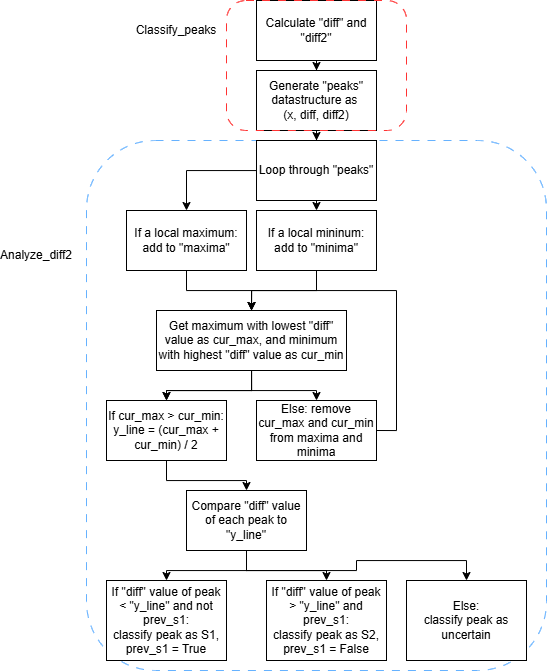
\includegraphics[width=0.8\textwidth]{docs/assignments/Midterm report/figures/module_1/classification_flowchart.png}
    \caption{Block diagram of the steps taken by the functions "classify\_peaks" and "analyze\_diff2".}  
    \label{fig:classificationchart}
\end{figure}

\begin{figure} [H]
    \centering
    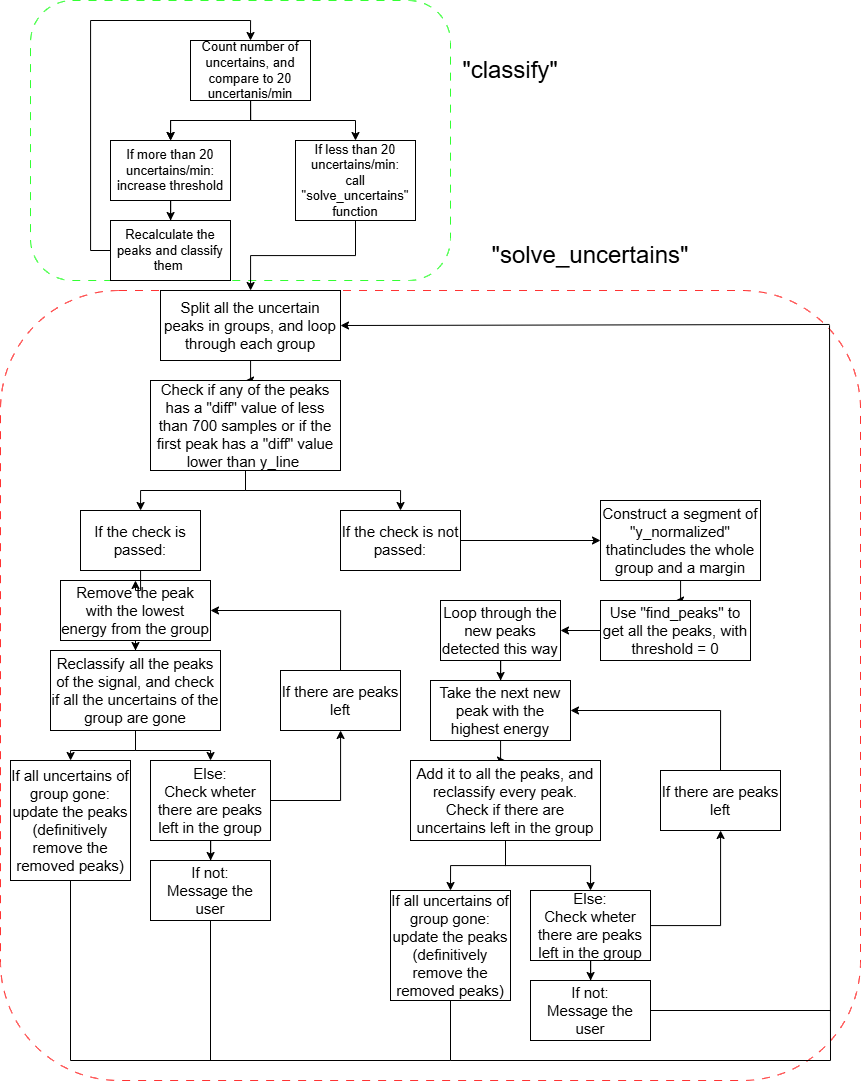
\includegraphics[width=0.8\textwidth]{docs/assignments/Midterm report/figures/module_1/solve_uncertains.png}
    \caption{Block diagram of the steps taken to increase the global threshold and the steps used by the function "solve\_uncertains".}  
    \label{fig:solve_uncertains_chart}
\end{figure}

\begin{figure} [H]
    \centering
    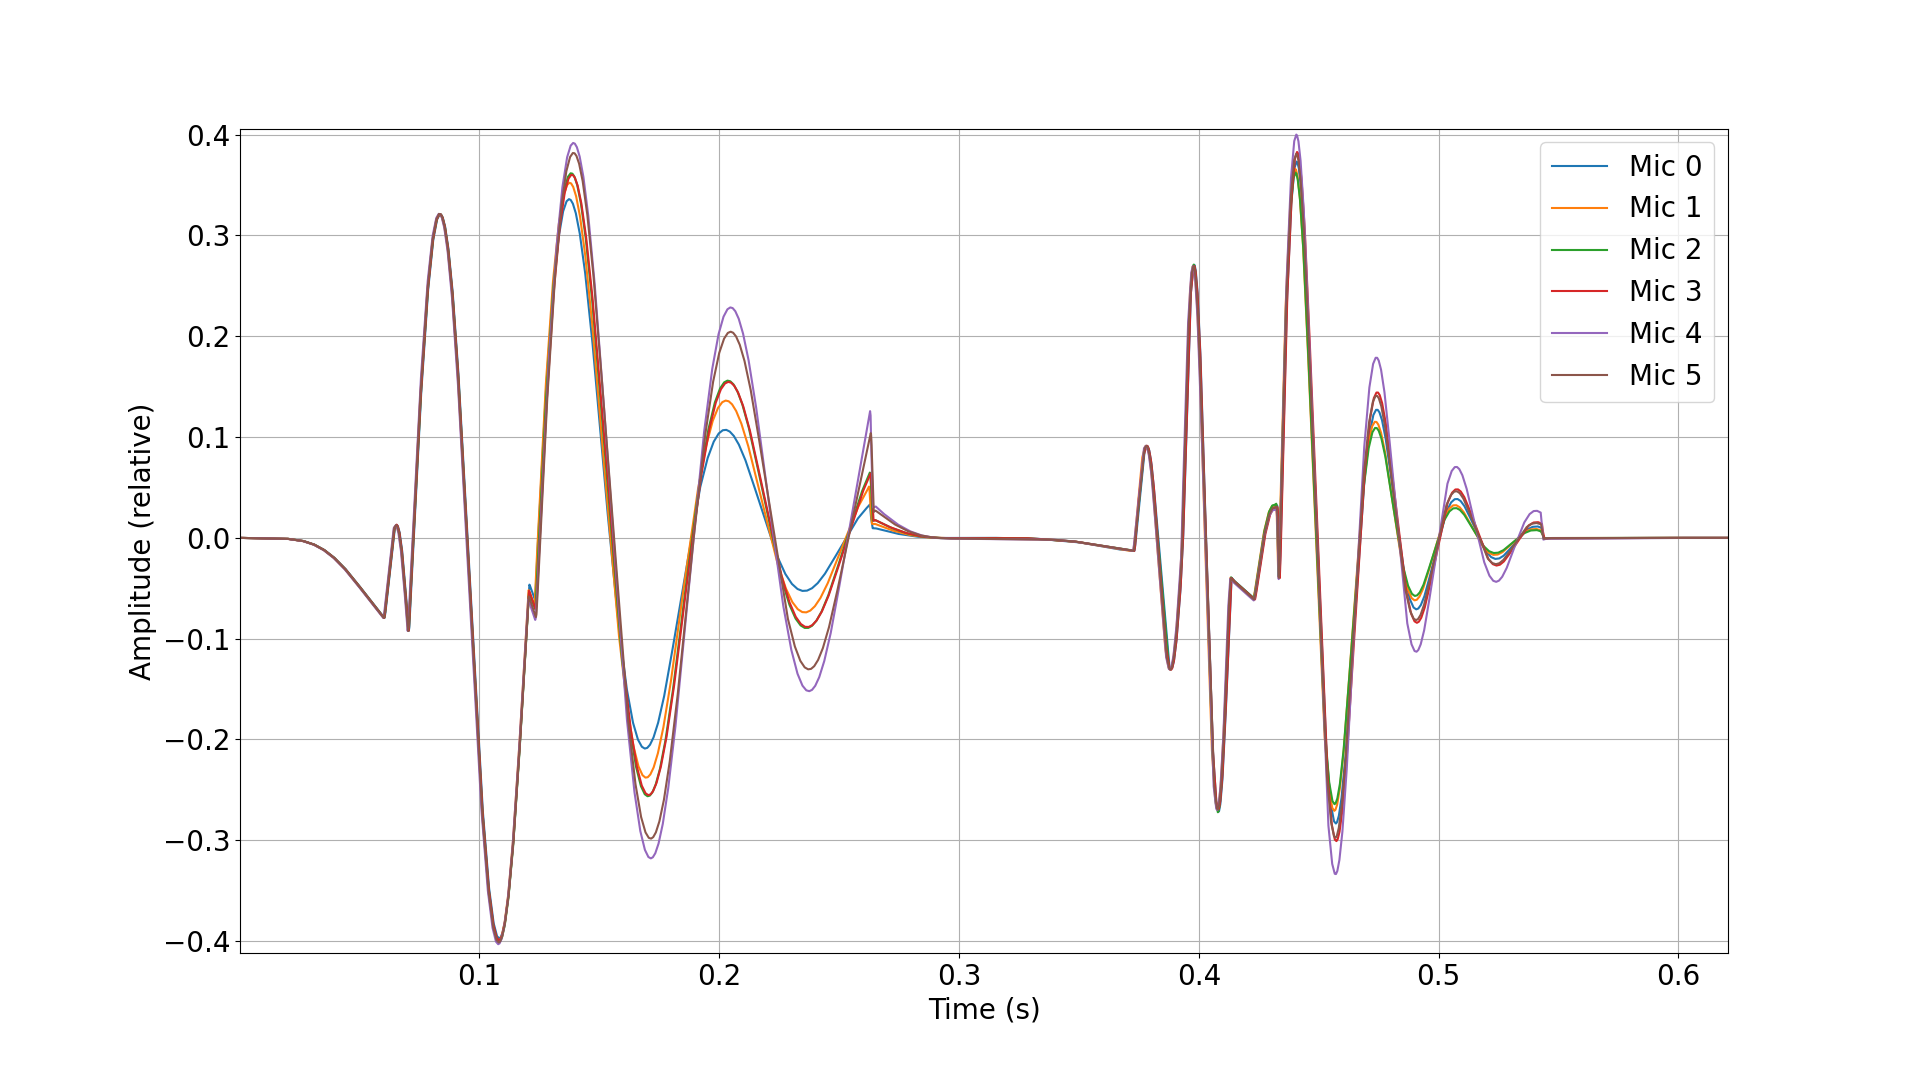
\includegraphics[width=0.8\textwidth]{docs/assignments/Midterm report/figures/module_2/multichannel_damping.png}
    \caption{Modeled signal for each microphone.}  
    \label{fig:multichannel_damping}
\end{figure}

\begin{figure} [H]
    \centering
    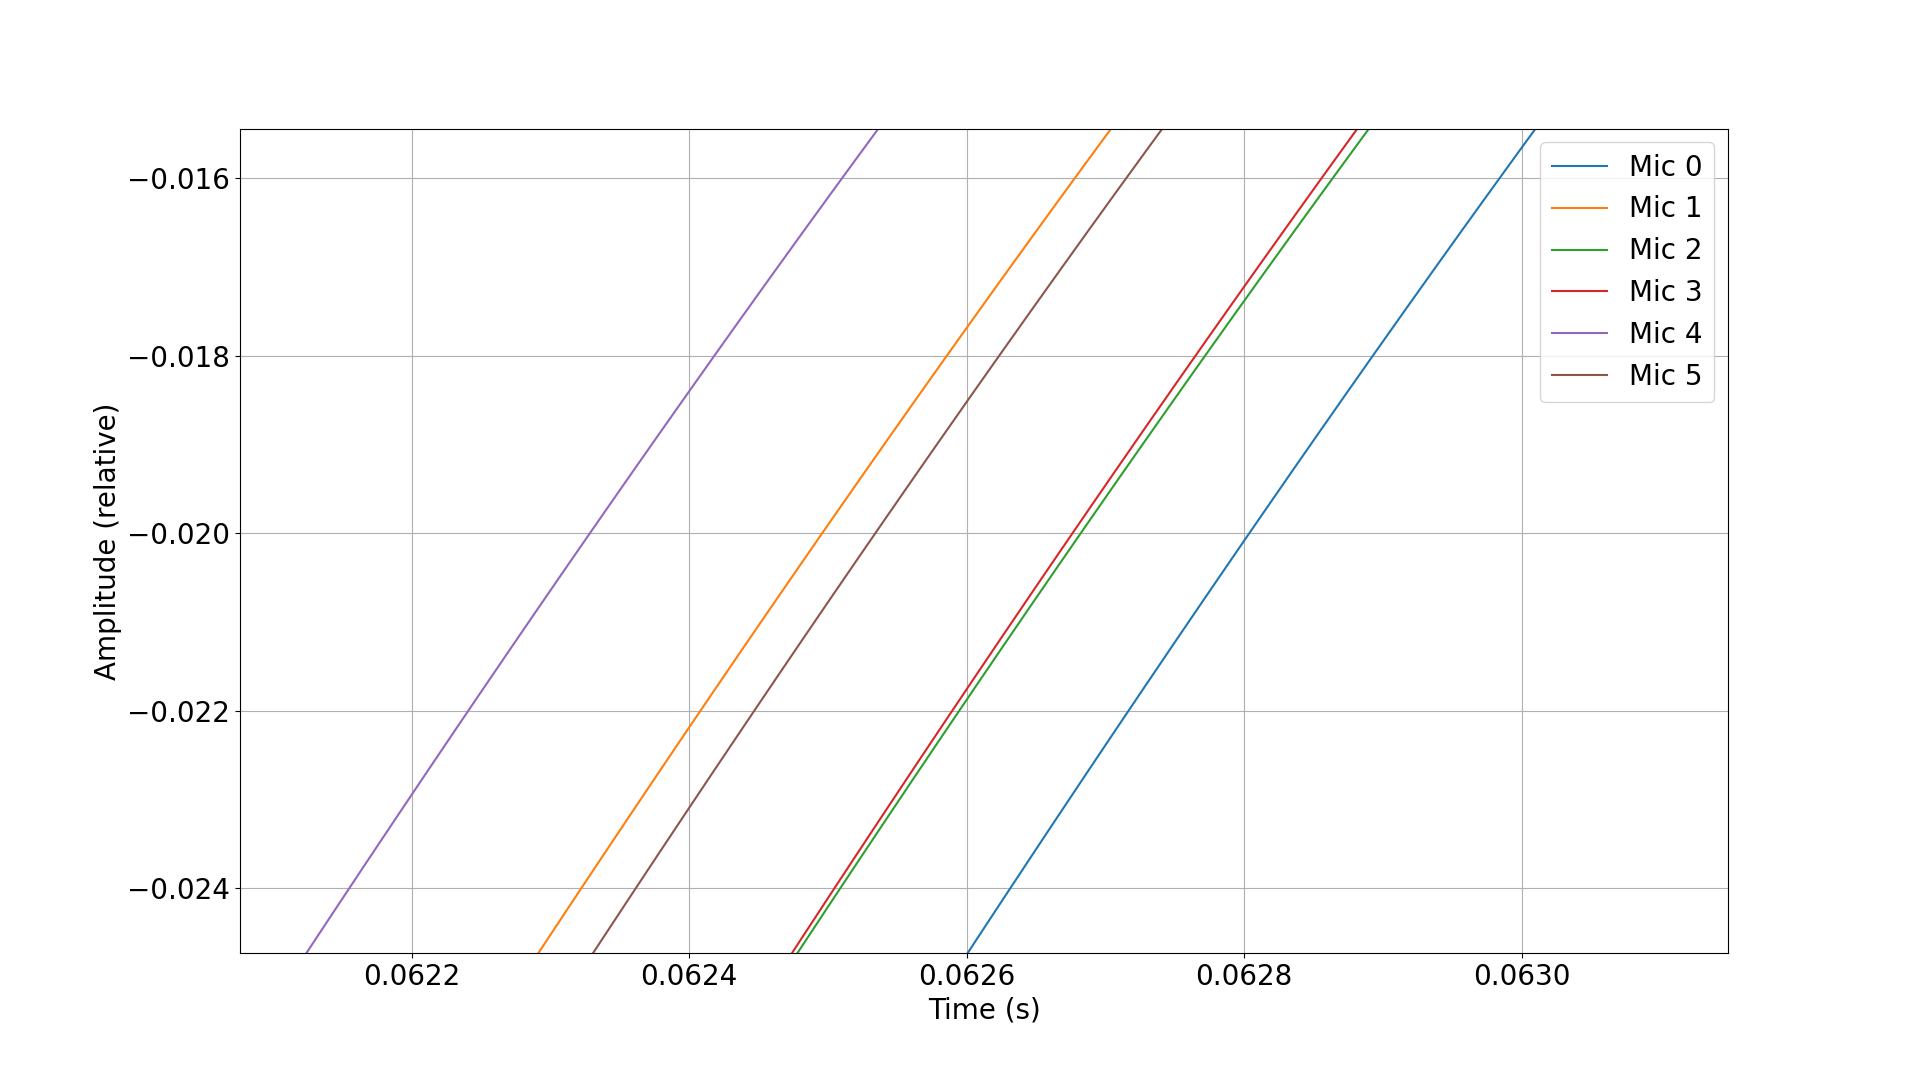
\includegraphics[width=0.8\textwidth]{docs/assignments/Midterm report/figures/module_2/multichannel_delay.png}
    \caption{Modeled signal for each microphone. Same data as Fig. \ref{fig:multichannel_damping}, but zoomed in.}  
    \label{fig:multichannel_delay}
\end{figure}


\begin{figure} [H]
    \centering
    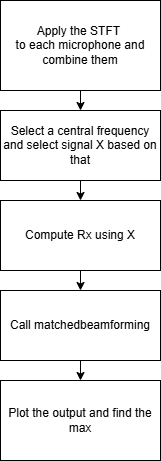
\includegraphics[width=0.3\textwidth]{docs/assignments/Midterm report/figures/module_3/Beamformer/beamforming_pipeline.png}
    \caption{Description of the beamformer pipeline.}  
    \label{fig:beamformer_pipeline}
\end{figure}

\chapter{Module 3 Calculations}


Calculation for central frequency.
Given the spacing $d = 0.1$ m and assuming the speed of sound $v = 343$ m/s:
\begin{equation}
    f = \frac{v}{2d} = \frac{343}{2 \cdot 0.1} = \frac{343}{0.2} = 1715 \text{ Hz}
\end{equation}
\label{module_3_calculation_central_frequency}

\chapter{Module 3 figures}

\begin{figure} [H]
    \centering
    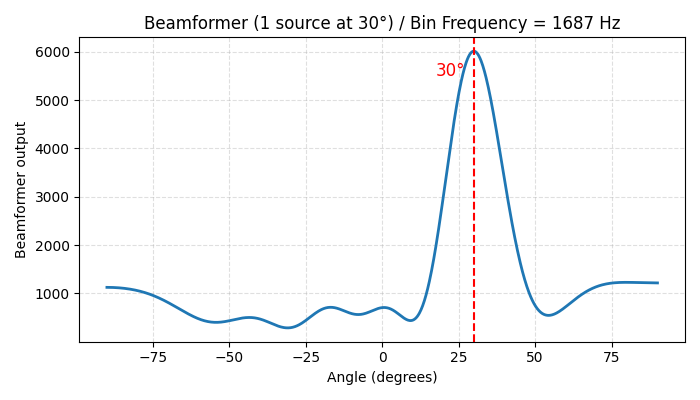
\includegraphics[width=0.8\textwidth]{docs/assignments/Midterm report/figures/module_3/Beamformer/Beamformer 1 source/Beamformer_30.png}
    \caption{Beamformer at $30^\circ$.}  
    \label{fig:beamformer_30_degrees}
\end{figure}

\begin{figure} [H]
    \centering
    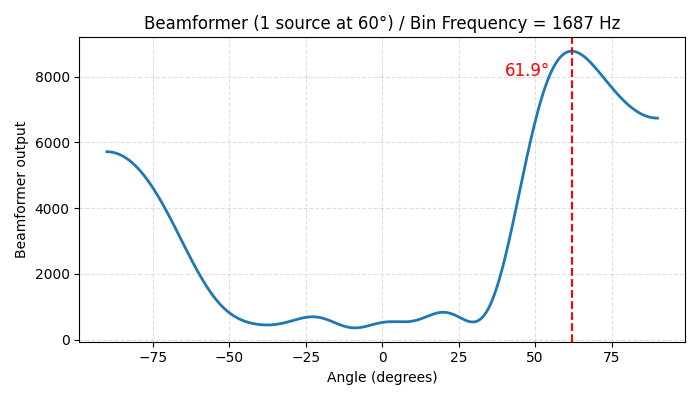
\includegraphics[width=0.8\textwidth]{docs/assignments/Midterm report/figures/module_3/Beamformer/Beamformer 1 source/Beamformer_60.png}
    \caption{Beamformer at $30^\circ$.}  
    \label{fig:beamformer_60_degrees}
\end{figure}


\begin{figure} [H]
    \centering
    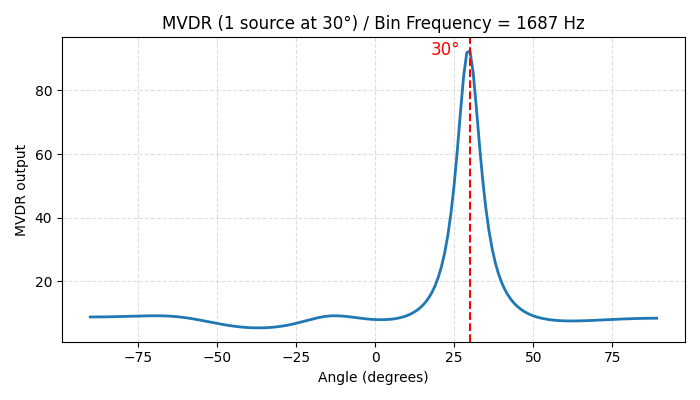
\includegraphics[width=0.8\textwidth]{docs/assignments/Midterm report/figures/module_3/MVDR/MVDR 1 source/MVDR_30.png}
    \caption{MVDR at $30^\circ$.}  
    \label{fig:MVDR_30_degrees}
\end{figure}

\begin{figure} [H]
    \centering
    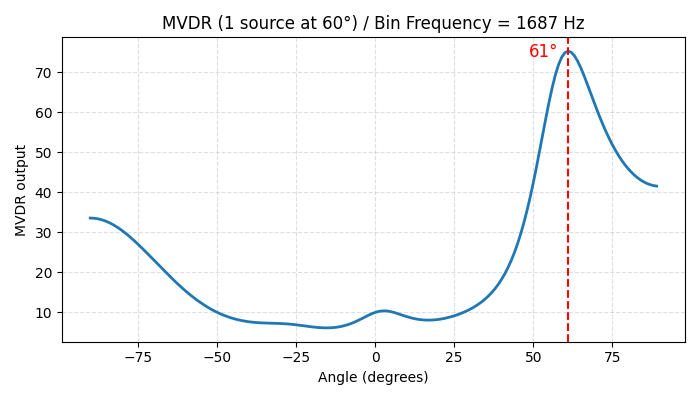
\includegraphics[width=0.8\textwidth]{docs/assignments/Midterm report/figures/module_3/MVDR/MVDR 1 source/MVDR_60.png}
    \caption{MVDR at $60^\circ$.}  
    \label{fig:MVDR_60_degrees}
\end{figure}



\chapter{Module 4 figures}
\begin{figure} [H]
    \centering
    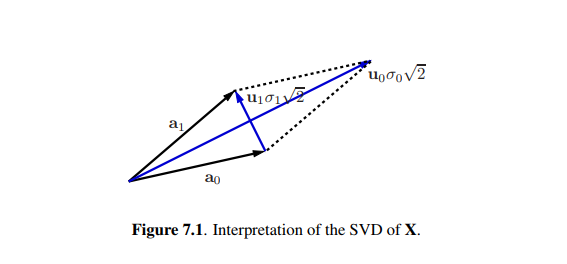
\includegraphics[width=0.8\textwidth]{docs/assignments/Midterm report/figures/module_4/SVD_explanation.png}
    \caption{SVD interpretation.}  
    \label{fig:SVD_interpretation}
\end{figure}

\begin{figure} [H]
    \centering
    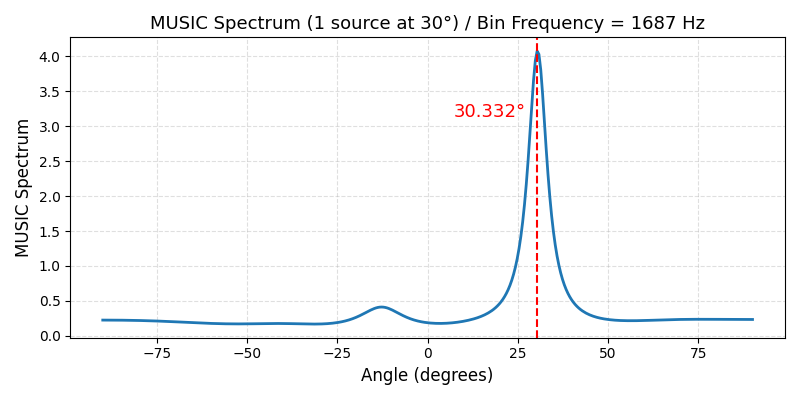
\includegraphics[width=0.8\textwidth]{docs/assignments/Midterm report/figures/module_4/MUSIC/MUSIC Single Source/Music_30_degrees.png}
    \caption{Beamformer at +7$^\circ$, -7$^\circ$, higher resolution.}  
    \label{fig:music_1_source_30_degrees}
\end{figure}

\begin{figure} [H]
    \centering
    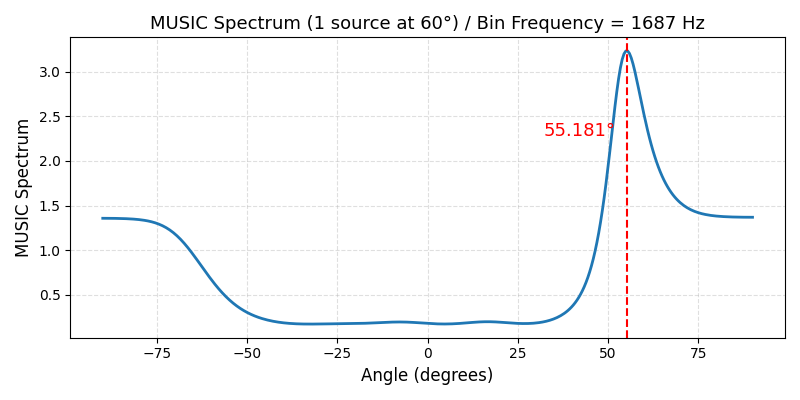
\includegraphics[width=0.8\textwidth]{docs/assignments/Midterm report/figures/module_4/MUSIC/MUSIC Single Source/Music_60_degrees.png}
    \caption{Beamformer at +7$^\circ$, -7$^\circ$, higher resolution.}  
    \label{fig:music_1_source_60_degrees}
\end{figure}


\begin{figure} [H]
    \centering
    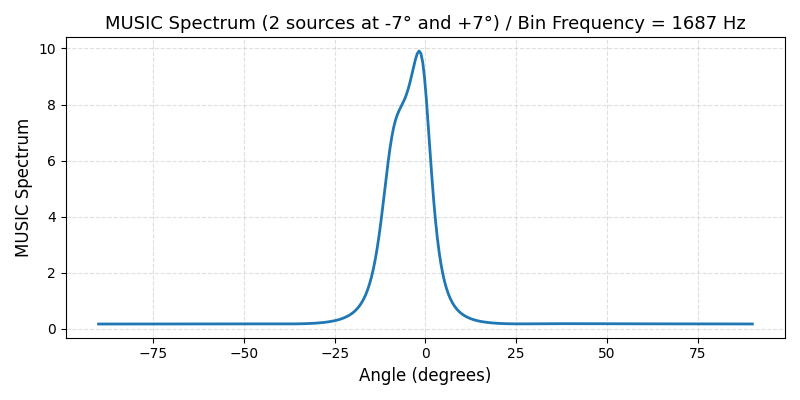
\includegraphics[width=0.8\textwidth]{docs/assignments/Midterm report/figures/module_4/MUSIC/MUSIC 2 sources/Bin freq = 1687 no dashed line.png}
    \caption{Beamformer at +7$^\circ$, -7$^\circ$, higher resolution.}  
    \label{fig:music_2_source_1687}
\end{figure}


\section{Assignments module 3 and 4}
\subsection{Assignment 6.2.3}
The function is created, and tested via printing and checking the complex numbers it gives.
\subsection{Assignment 6.2.6}
\label{assigment_6.2.6}
For direction of arrival at $0^\circ$, $M = 7$, $f = 500\text{Hz}$, 
and $v = 340\text{m/s}$, the following plots have been acquired. 
It is obvious that the resolution increases (sharper lobes) but 
aliasing is introduced with increasing $\Delta$.

\begin{figure} [H]
    \centering
    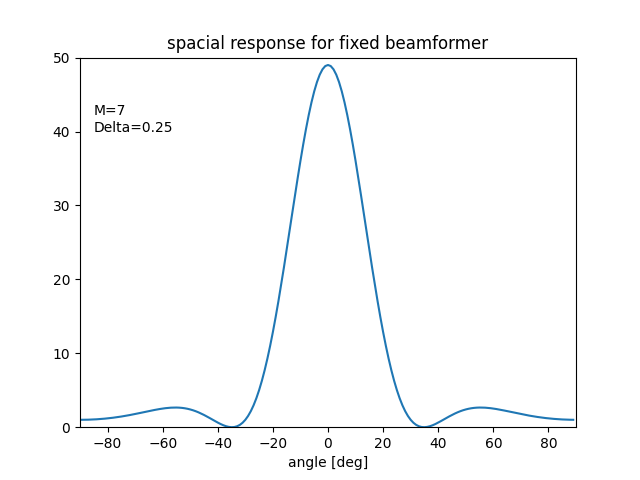
\includegraphics[width=0.8\textwidth]{docs/assignments/Midterm report/figures/Assignments/assignment_6.2.6.1.png}
    \caption{}  
    \label{fig:assignment_6.2.6.1}
\end{figure}

\begin{figure} [H]
    \centering
    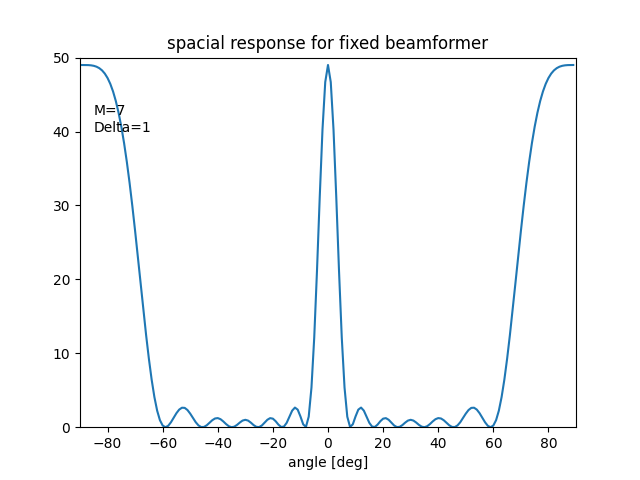
\includegraphics[width=0.8\textwidth]{docs/assignments/Midterm report/figures/Assignments/assignment_6.2.6.2.png}
    \caption{}  
    \label{fig:assignment_6.2.6.2}
\end{figure}

\begin{figure} [H]
    \centering
    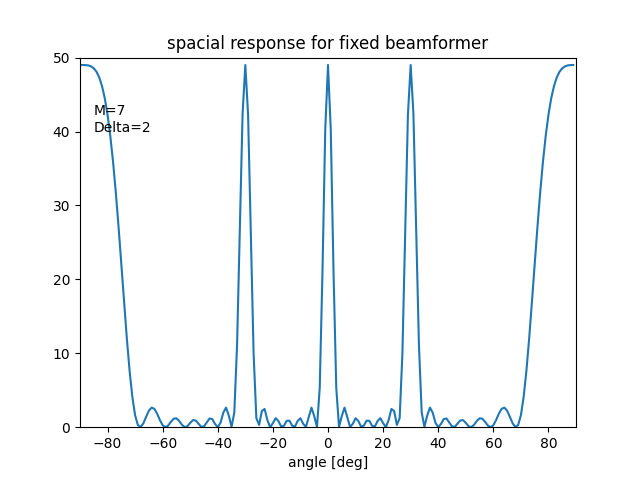
\includegraphics[width=0.8\textwidth]{docs/assignments/Midterm report/figures/Assignments/assignment_6.2.6.3.png}
    \caption{}  
    \label{fig:assignment_6.2.6.3}
\end{figure}


For a different angle , e.g. $30^\circ$, the following plots were obtained, confirming that aliasing might lead to misleading information.

\begin{figure} [H]
    \centering
    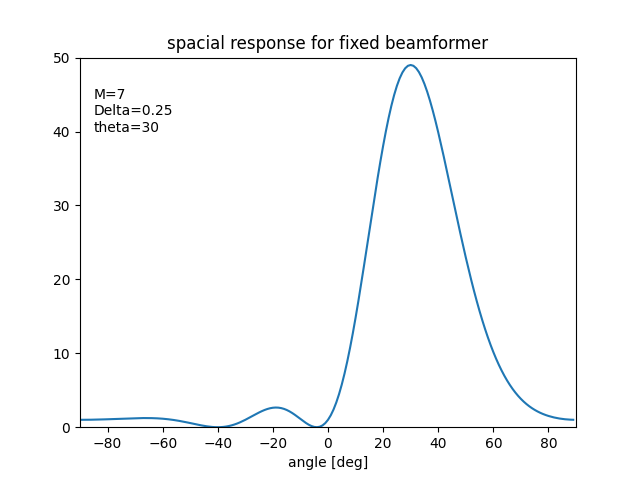
\includegraphics[width=0.8\textwidth]{docs/assignments/Midterm report/figures/Assignments/Assigment 6.2.6/30 degrees.png}
    \caption{}  
    \label{fig:assignment_6.2.6.30a}
\end{figure}

\begin{figure} [H]
    \centering
    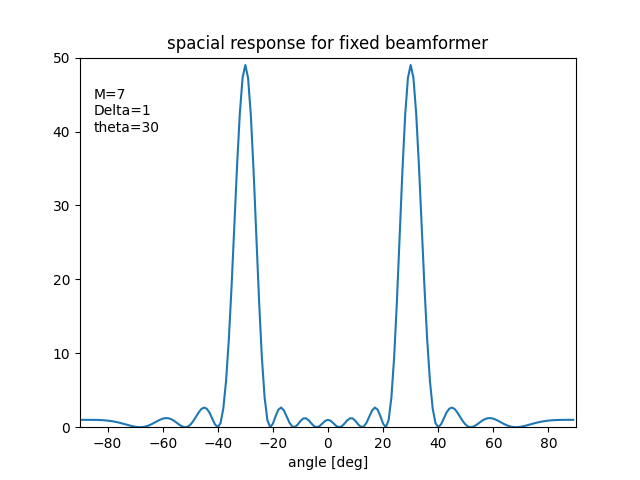
\includegraphics[width=0.8\textwidth]{docs/assignments/Midterm report/figures/Assignments/Assigment 6.2.6/30 degrees 2.png}
    \caption{}  
    \label{fig:assignment_6.2.6.30b}
\end{figure}

\begin{figure} [H]
    \centering
    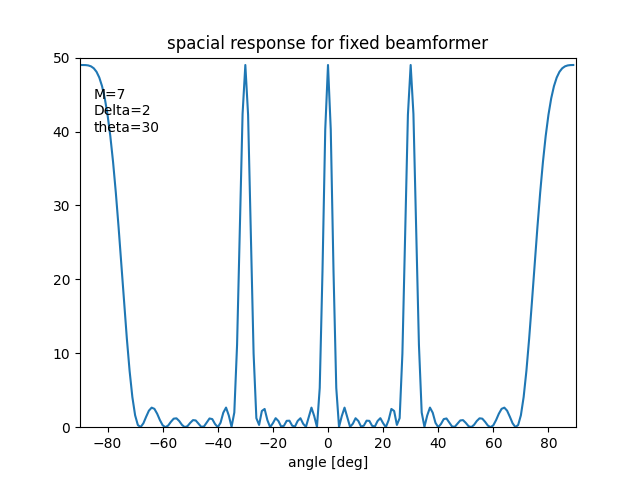
\includegraphics[width=0.8\textwidth]{docs/assignments/Midterm report/figures/Assignments/Assigment 6.2.6/30 degrees 3.png}
    \caption{}  
    \label{fig:assignment_6.2.6.30c}
\end{figure}


\subsection{Assignment 6.2.9}

\begin{enumerate}
    \item \textbf{Narrowband Condition (Linear Array)} \\
    The text states the condition is $B \ll v/D$, where $D = (M-1)d$. \\
    Given: $M=6$, $d=0.1$ m, $v \approx 340$ m/s (speed of sound).
    $$ D = (6-1)(0.1) = 0.5 \text{ m} $$
    $$ B \ll \frac{340}{0.5} = 680 \text{ Hz} $$
    
    \item \textbf{Minimal Spacing for Spatial Aliasing} \\
    The text states we need $\Delta < 1/2$, which means $d < \lambda/2$. \\
    Given: $F_0 = 1000$ Hz.
    $$ \lambda = \frac{v}{F_0} = \frac{340}{1000} = 0.34 \text{ m} $$
    $$ d < \frac{0.34}{2} = 0.17 \text{ m} $$
    The spacing must be less than 17 cm.

    \item \textbf{Heart Sound Array ($2 \times 3$)} \\
    We need $B \ll v_{body}/D_{max}$. \\
    Given: Spacing $d=0.05$ m, $v_{body} = 60$ m/s. \\
    The array is 2 rows by 3 columns. The max distance $D$ is the diagonal from corner to corner.
    $$ \text{Width} = (3-1)d = 2d, \quad \text{Height} = (2-1)d = 1d $$
    $$ D = \sqrt{(2d)^2 + (d)^2} = d\sqrt{5} \approx 0.05 \times 2.236 = 0.112 \text{ m} $$
    $$ B \ll \frac{60}{0.112} \approx 536 \text{ Hz} $$

    \item \textbf{Physical Reason for $\Delta$} \\
    $\Delta = d/\lambda$ represents the sampling density in space.
    \begin{itemize}
        \item \textbf{Smaller $\Delta$:} Samples are very close. This reduces the phase difference between microphones, making the main lobe wider (worse resolution).
        \item \textbf{Larger $\Delta$:} Samples are far apart. This improves resolution (sharper lobe), but if $\Delta > 0.5$, the sensors are too far apart to distinguish the wave cycle uniquely (undersampling), causing spatial aliasing (false peaks).
    \end{itemize}
\end{enumerate}

\subsection{Assignment 6.4.1}
\label{Assignment_6.4.1}
The functions in the code appendix have been implemented and the following plots were created. There are 2 sources at $0^\circ$ and $15^\circ$.

\begin{figure} [H]
    \centering
    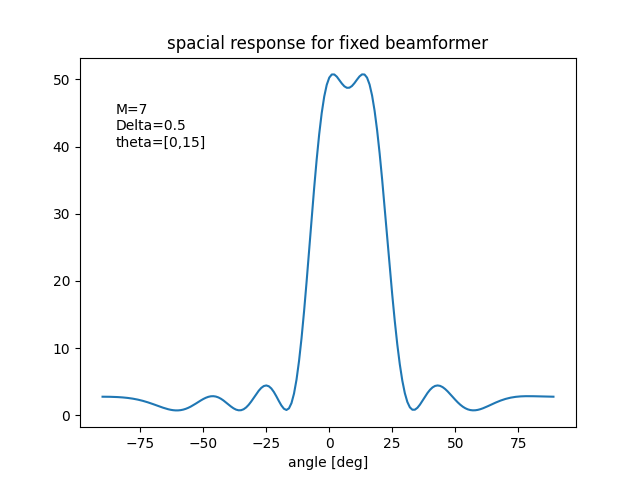
\includegraphics[width=0.8\textwidth]{docs/assignments/Midterm report/figures/Assignments/Assigment 6.4.1/matched_beamformer.png}
    \caption{}  
    \label{fig:assignment_6.4.1_beamformer}
\end{figure}

\begin{figure} [H]
    \centering
    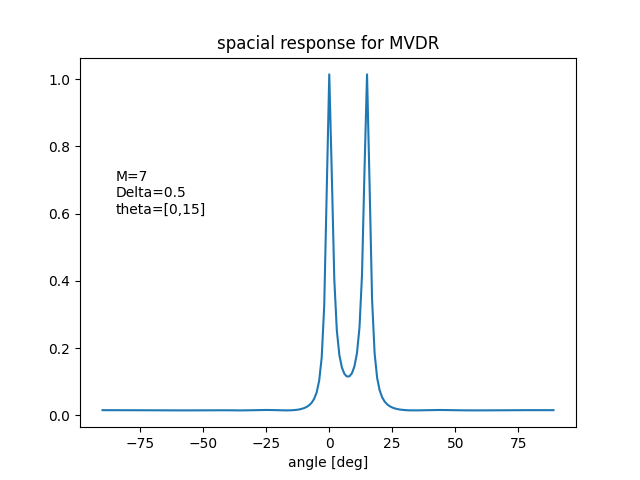
\includegraphics[width=0.8\textwidth]{docs/assignments/Midterm report/figures/Assignments/Assigment 6.4.1/MVDR.png}
    \caption{}  
    \label{fig:assignment_6.4.1_MVDR}
\end{figure}

\begin{figure} [H]
    \centering
    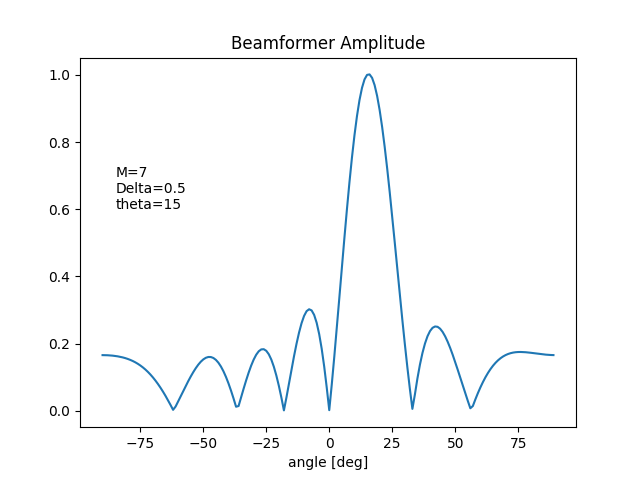
\includegraphics[width=0.8\textwidth]{docs/assignments/Midterm report/figures/Assignments/Assigment 6.4.1/MVDR beamformer.png}
    \caption{}  
    \label{fig:assignment_6.4.1_MVDR_beamformer}
\end{figure}

It is clear that given the angle $15^\circ$ the MVDR beamformer has a zero response/amplitude in the direction of the other source at $0^\circ$.


\subsection{Assignment 6.6.2}
The first part of this assignment was implemented a bit differently. First there was a central frequency that was chosen. Then this resulted in a signal \textbf{X} which would be M x N and computing the auto covariance could be done with np.cov(X). The implementation is visible in the code appendix


\subsection {Assignment 7.1.4}
The following plot was created. There are three sources at $10^\circ$, $90^\circ$ and $60^\circ$
\begin{figure} [H]
    \centering
    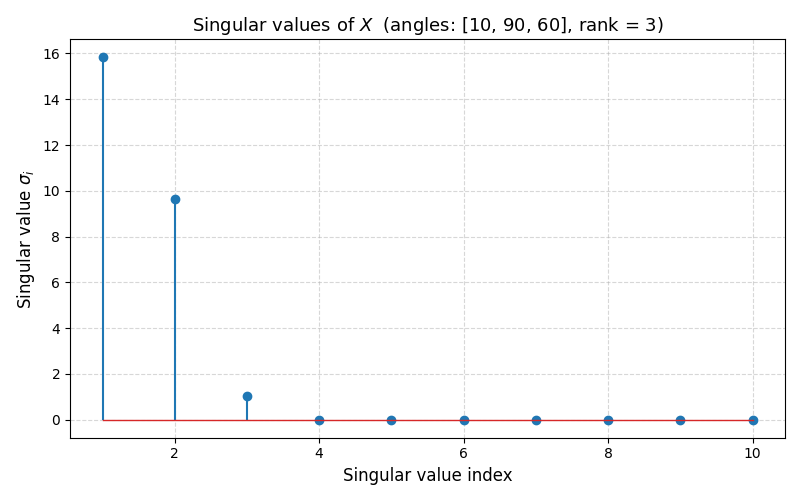
\includegraphics[width=0.8\textwidth]{docs/assignments/Midterm report/figures/Assignments/assigment_7.1.4.png}
    \caption{}  
    \label{fig:assignment_7.1.4_plot}
\end{figure}
This verifies that the number of non zero singular values is the same as the rank of the matrix \textbf{X}. 

\subsection{Assignment 7.2.1}
\begin{itemize}
\item Narrowband assumption: each source is treated as a single frequency so delays become simple phase shifts, while real signals are wideband.
\item Far-field (plane-wave) assumption: the source is assumed to be far away, but in practice it can be in the near field.
\item No reflections or multipath: only a direct path is assumed, while real environments contain echoes and reflections.
\item Ideal microphones and geometry: microphones are assumed identical and perfectly positioned, which is not true in practice.
\item Simple noise model: noise is assumed additive and uncorrelated, whereas real noise can be colored and correlated across microphones.
\end{itemize}


\subsection{Module 3 recordings}
\label{module_3_recordings}
Generally whenever the angle is measured to be e.g $-15^\circ$ the actual angle is $15^\circ$. This is because the microphone array was rotated in place of the source. 


\paragraph{For beamforming}
\begin{figure} [H]
    \centering
    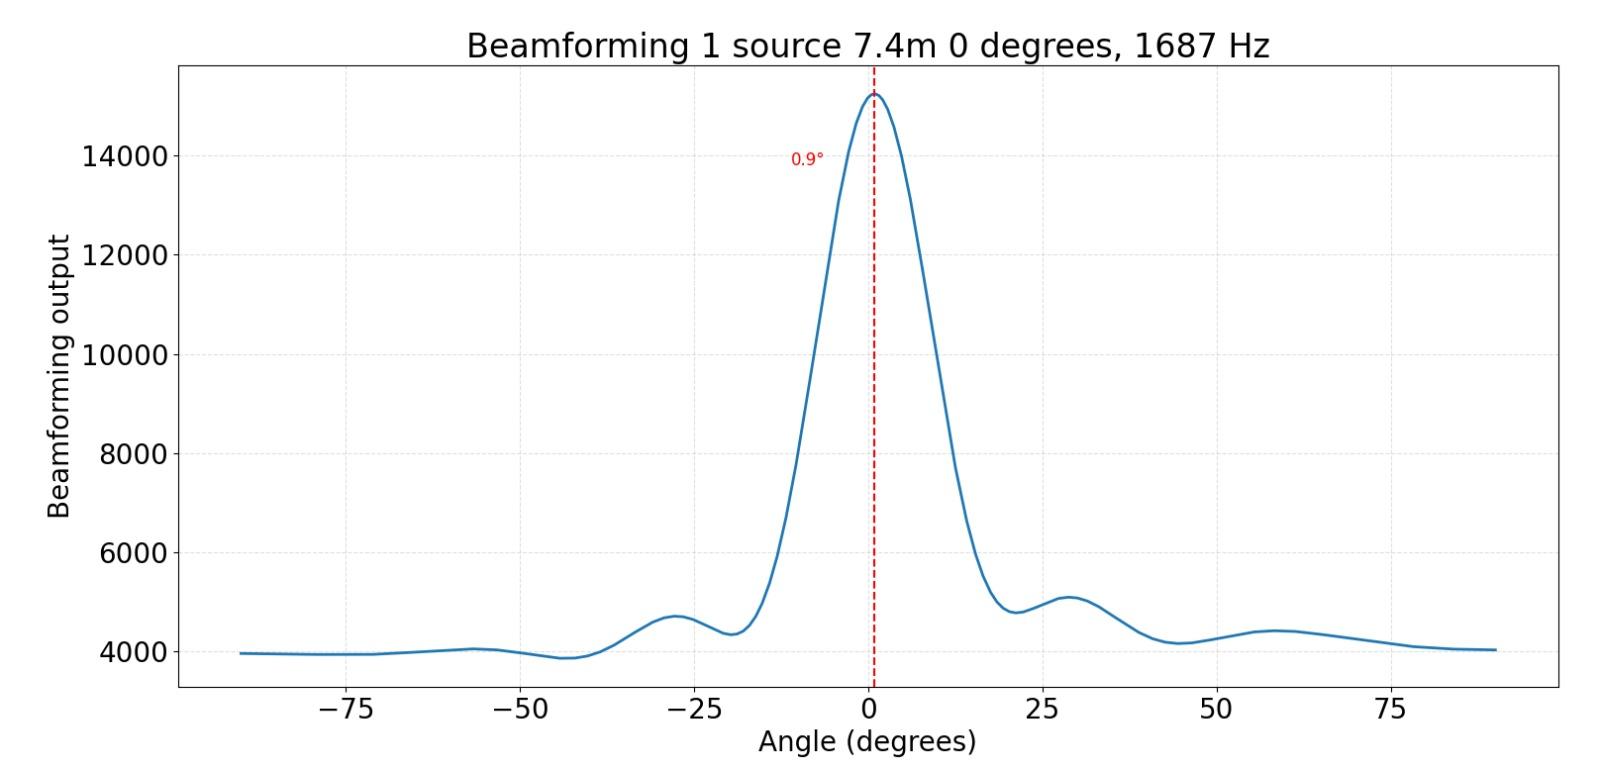
\includegraphics[width=0.9\textwidth]{docs/assignments/Midterm report/figures/Beamforming/1 source/0 degrees.jpg}
    \caption{}  
    \label{fig:beam1}
\end{figure}

\begin{figure} [H]
    \centering
    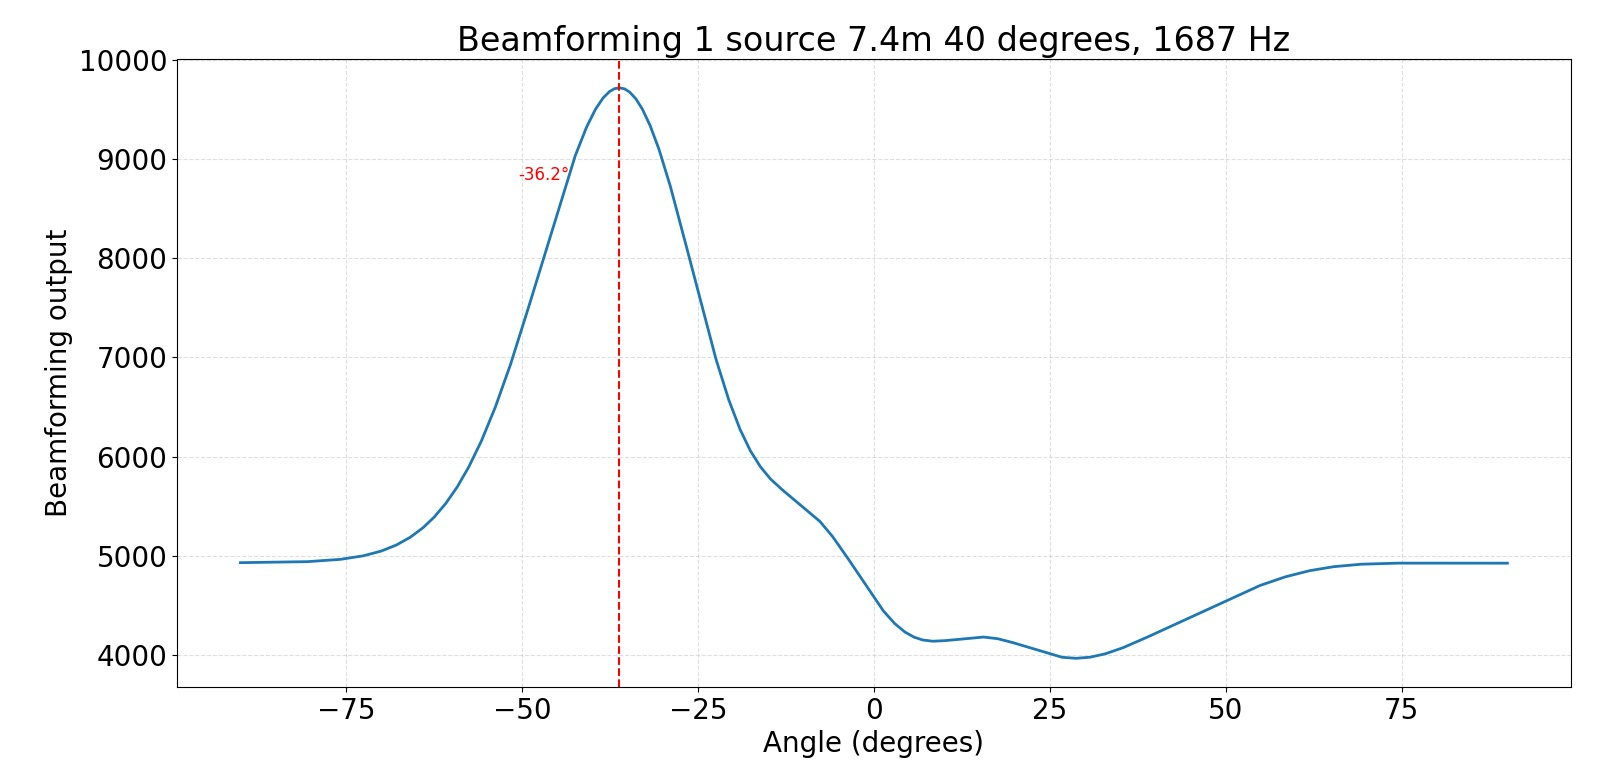
\includegraphics[width=0.8\textwidth]{docs/assignments/Midterm report/figures/Beamforming/1 source/40 degrees.jpg}
    \caption{}  
    \label{fig:beam3}
\end{figure}

\begin{figure} [H]
    \centering
    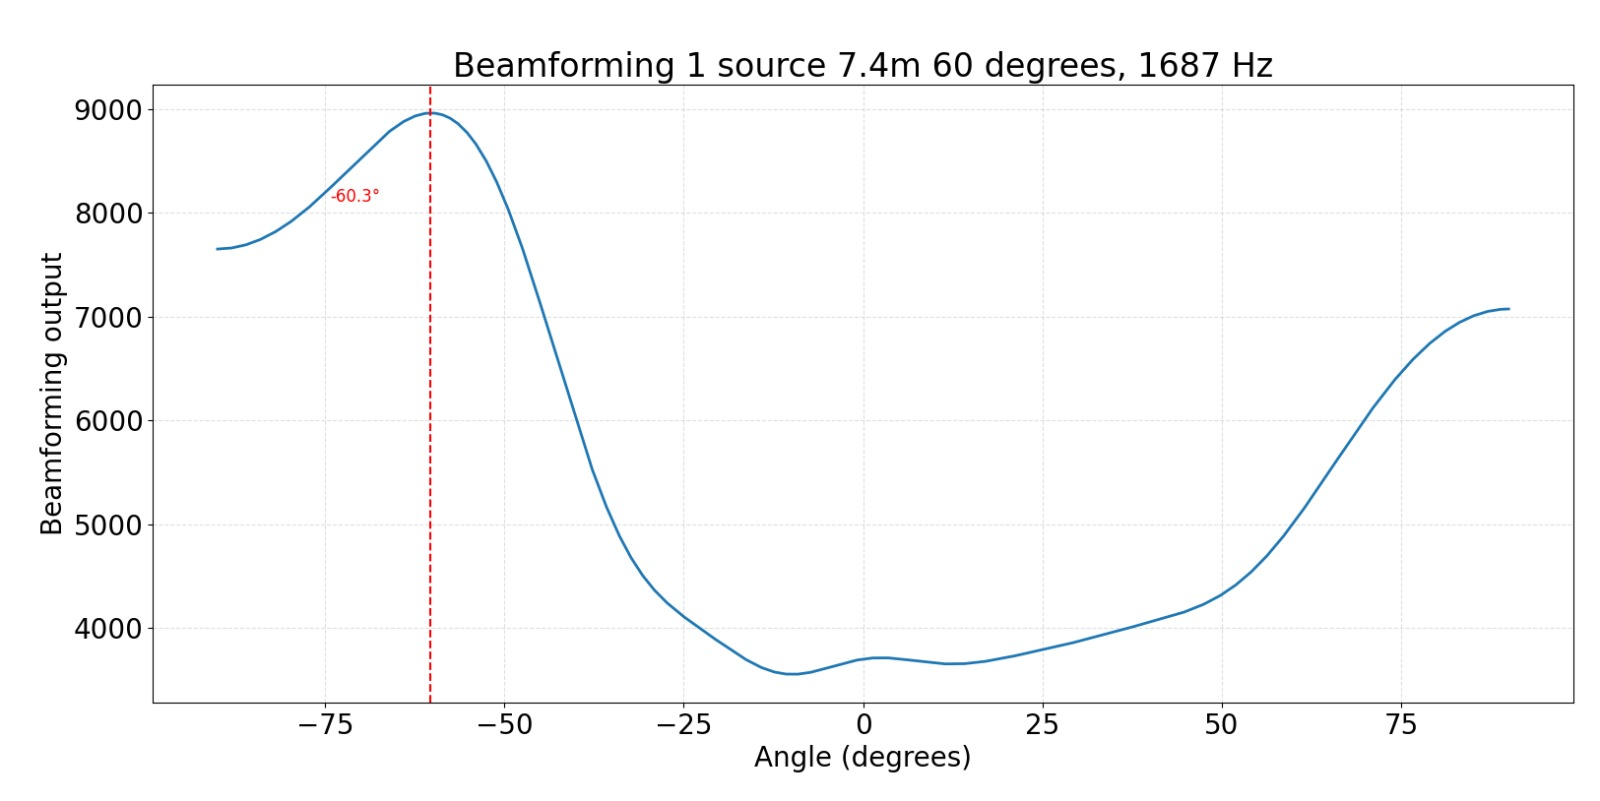
\includegraphics[width=0.8\textwidth]{docs/assignments/Midterm report/figures/Beamforming/1 source/60 degrees.jpg}
    \caption{}  
    \label{fig:beam4}
\end{figure}

\begin{figure} [H]
    \centering
    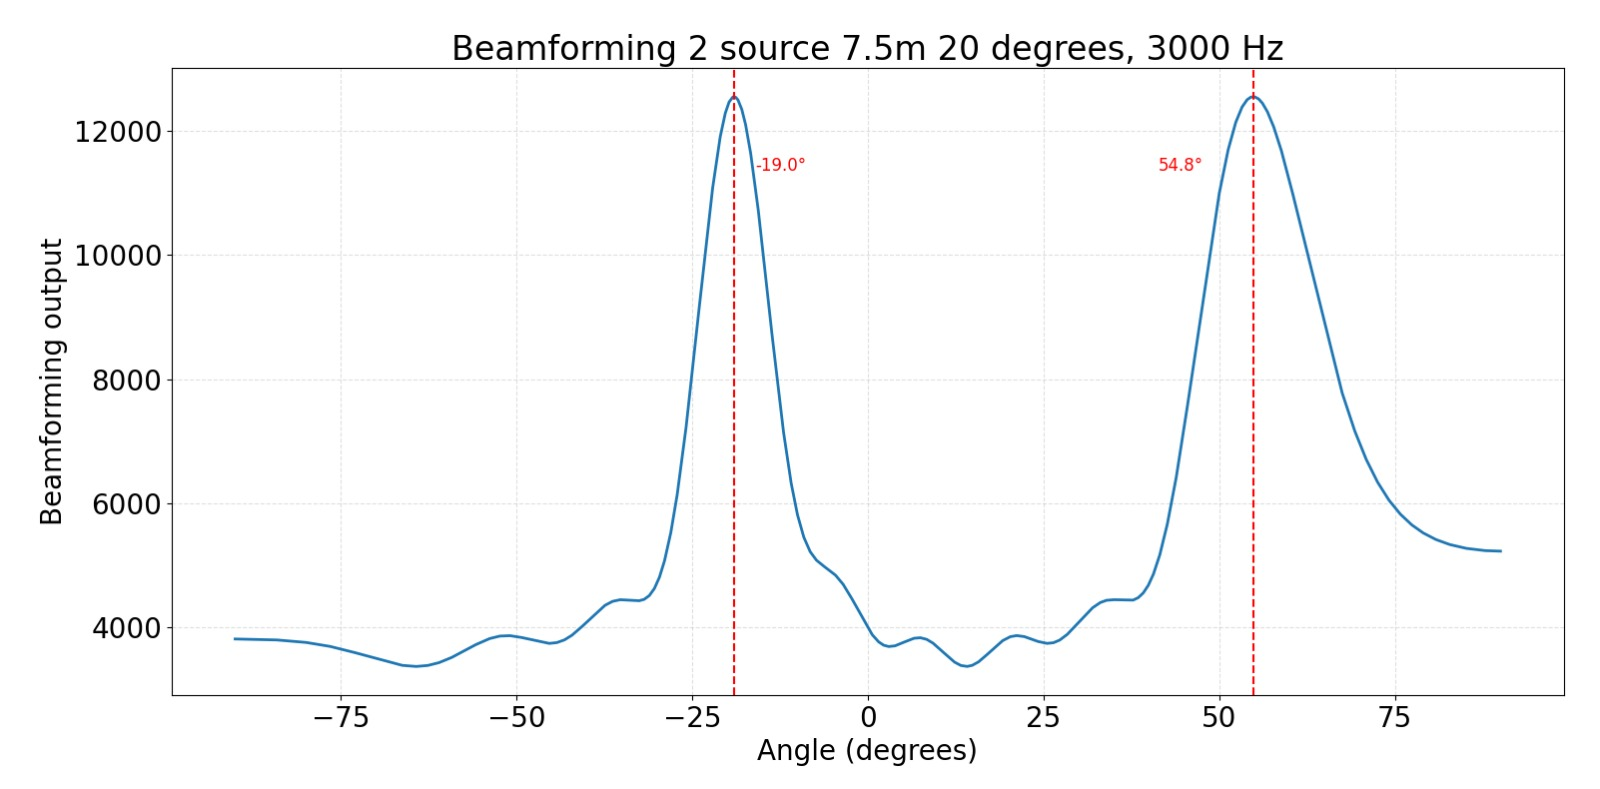
\includegraphics[width=0.8\textwidth]{docs/assignments/Midterm report/figures/Beamforming/2 source/20 degrees.jpg}
    \caption{}  
    \label{fig:beam5}
\end{figure}

\begin{figure} [H]
    \centering
    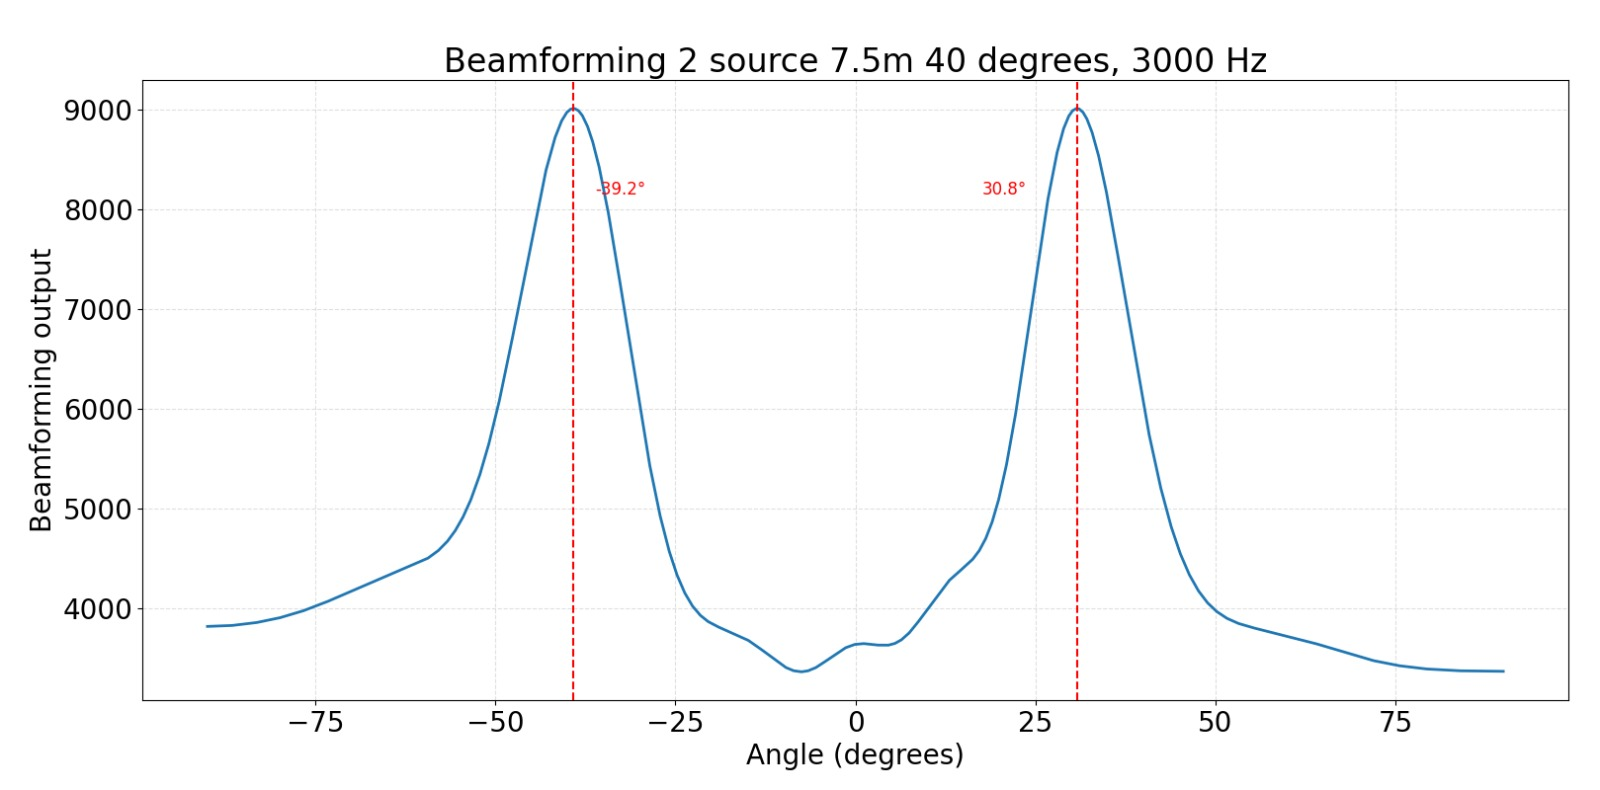
\includegraphics[width=0.8\textwidth]{docs/assignments/Midterm report/figures/Beamforming/2 source/40 degrees.jpg}
    \caption{}  
    \label{fig:beam6}
\end{figure}

\begin{figure} [H]
    \centering
    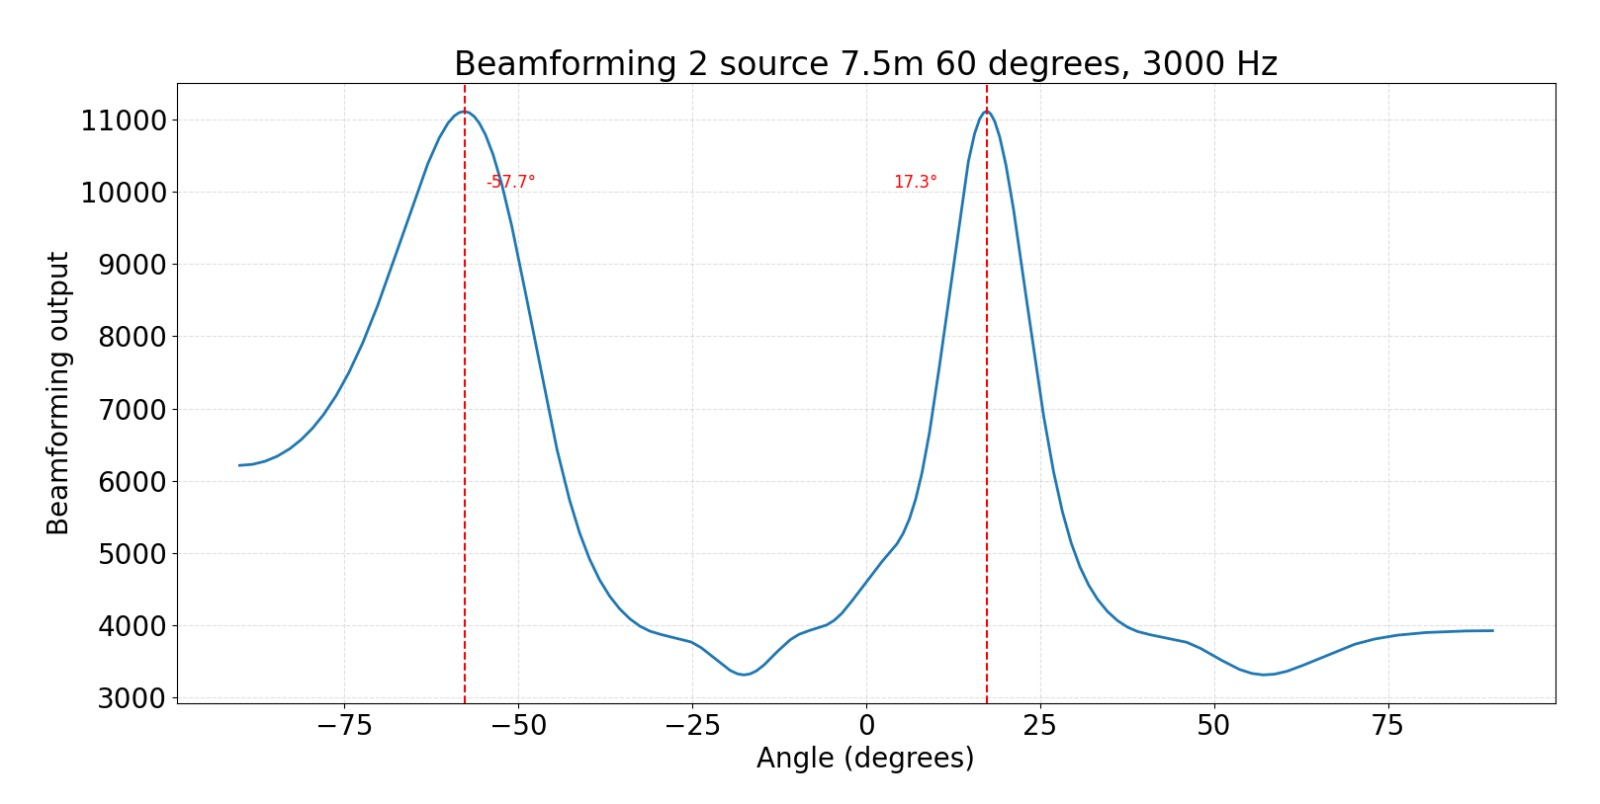
\includegraphics[width=0.8\textwidth]{docs/assignments/Midterm report/figures/Beamforming/2 source/60 degrees.jpg}
    \caption{}  
    \label{fig:beam7}
\end{figure}




\begin{figure} [H]
    \centering
    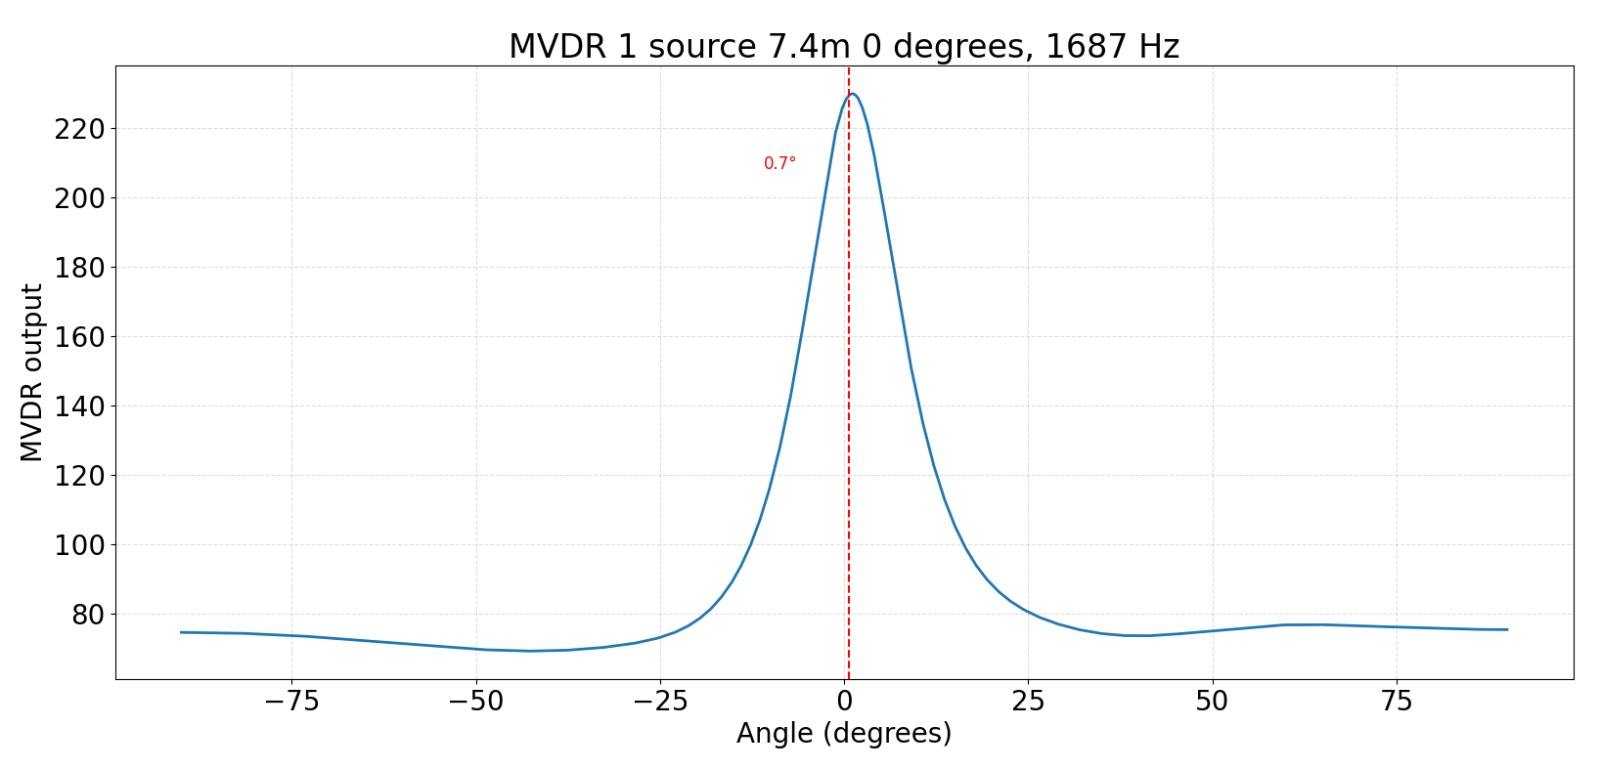
\includegraphics[width=0.8\textwidth]{docs/assignments/Midterm report/figures/MVDR/1 source/0 degrees.jpg}
    \caption{}  
    \label{fig:MVDR1}
\end{figure}


\begin{figure} [H]
    \centering
    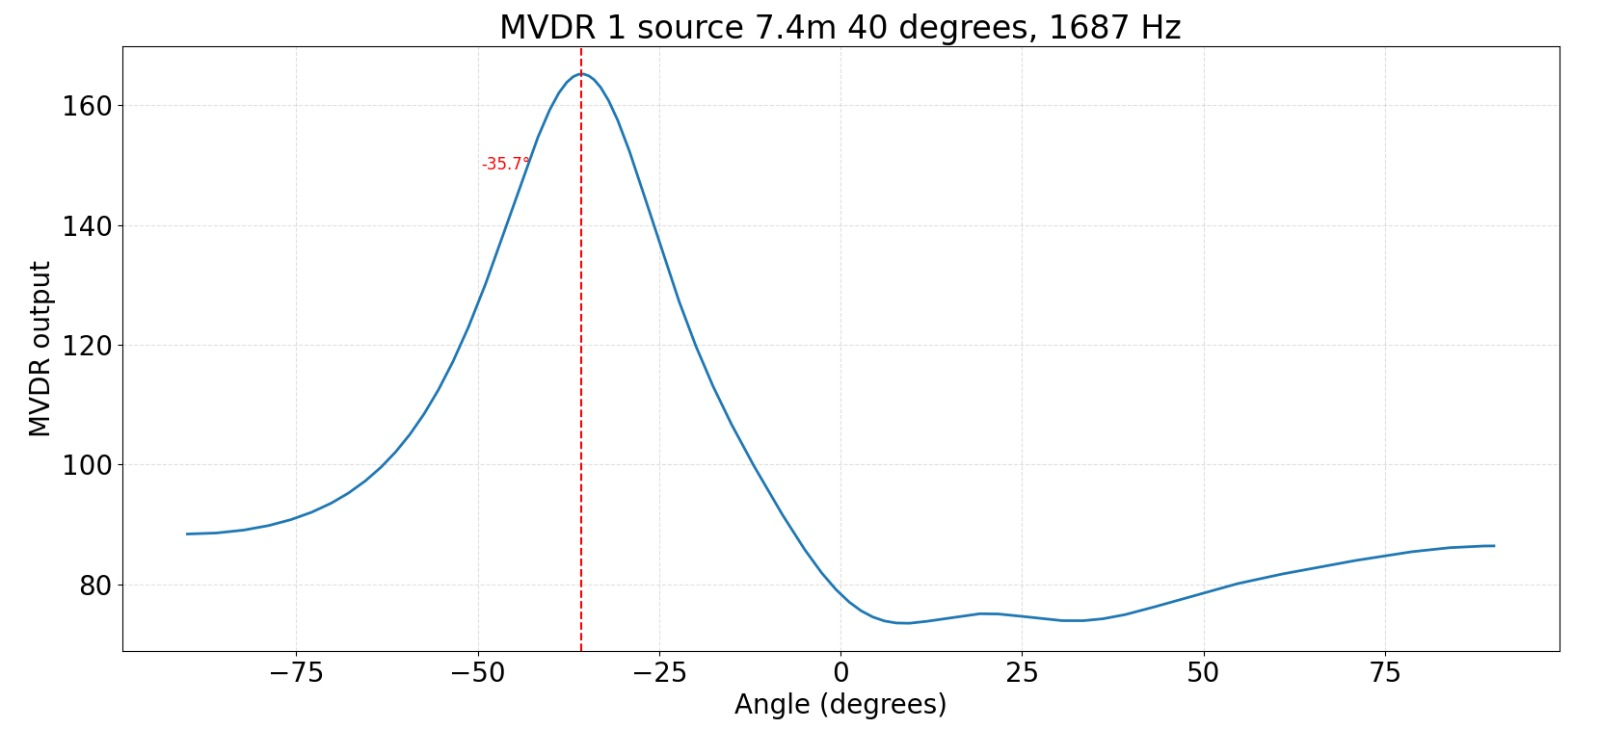
\includegraphics[width=0.8\textwidth]{docs/assignments/Midterm report/figures/MVDR/1 source/40 degrees.jpg}
    \caption{}  
    \label{fig:MVDR2}
\end{figure}

\begin{figure} [H]
    \centering
    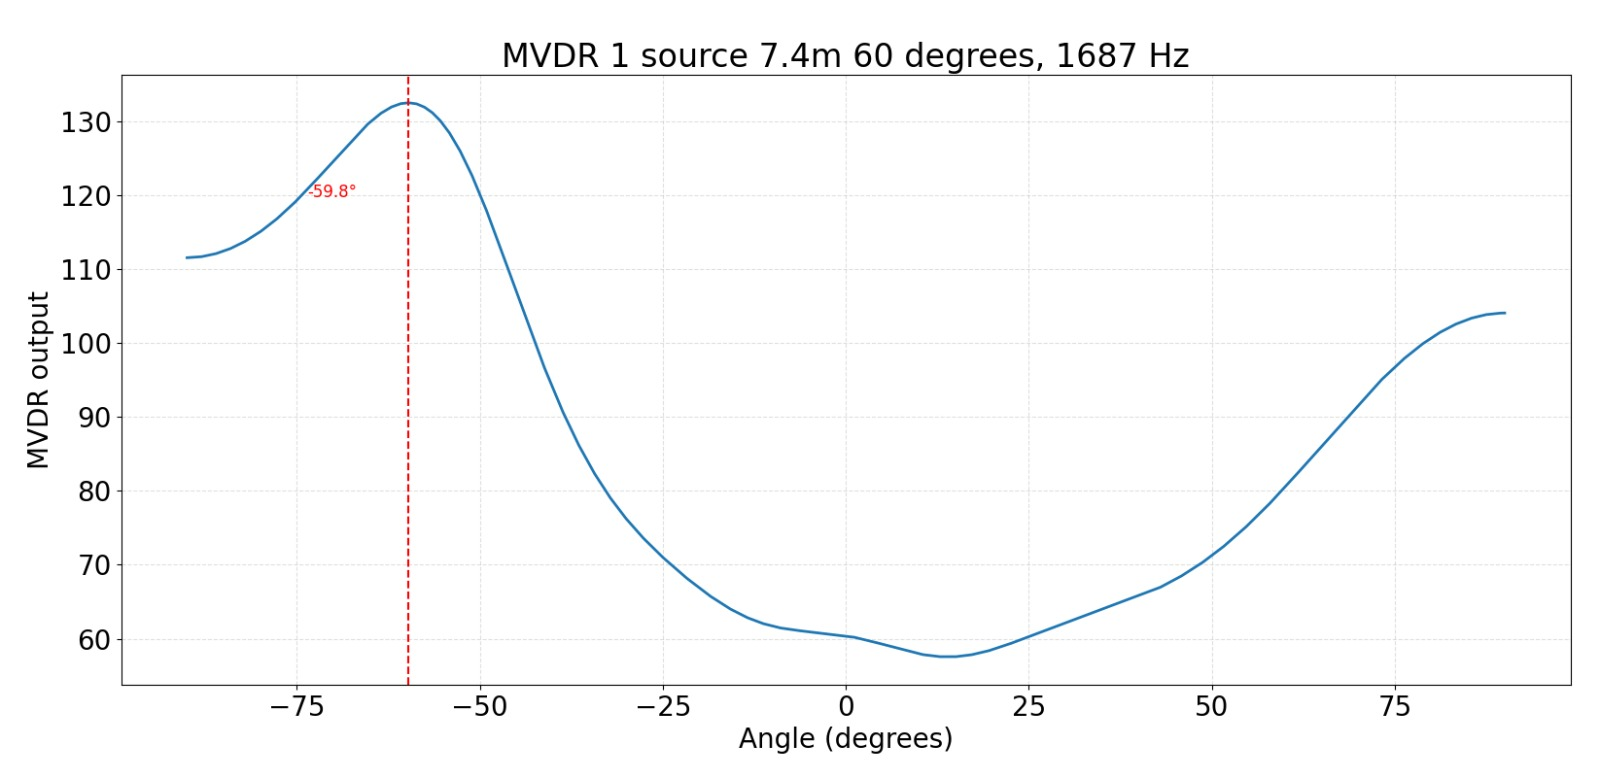
\includegraphics[width=0.8\textwidth]{docs/assignments/Midterm report/figures/MVDR/1 source/60 degrees.jpg}
    \caption{}  
    \label{fig:MVDR3}
\end{figure}

\begin{figure} [H]
    \centering
    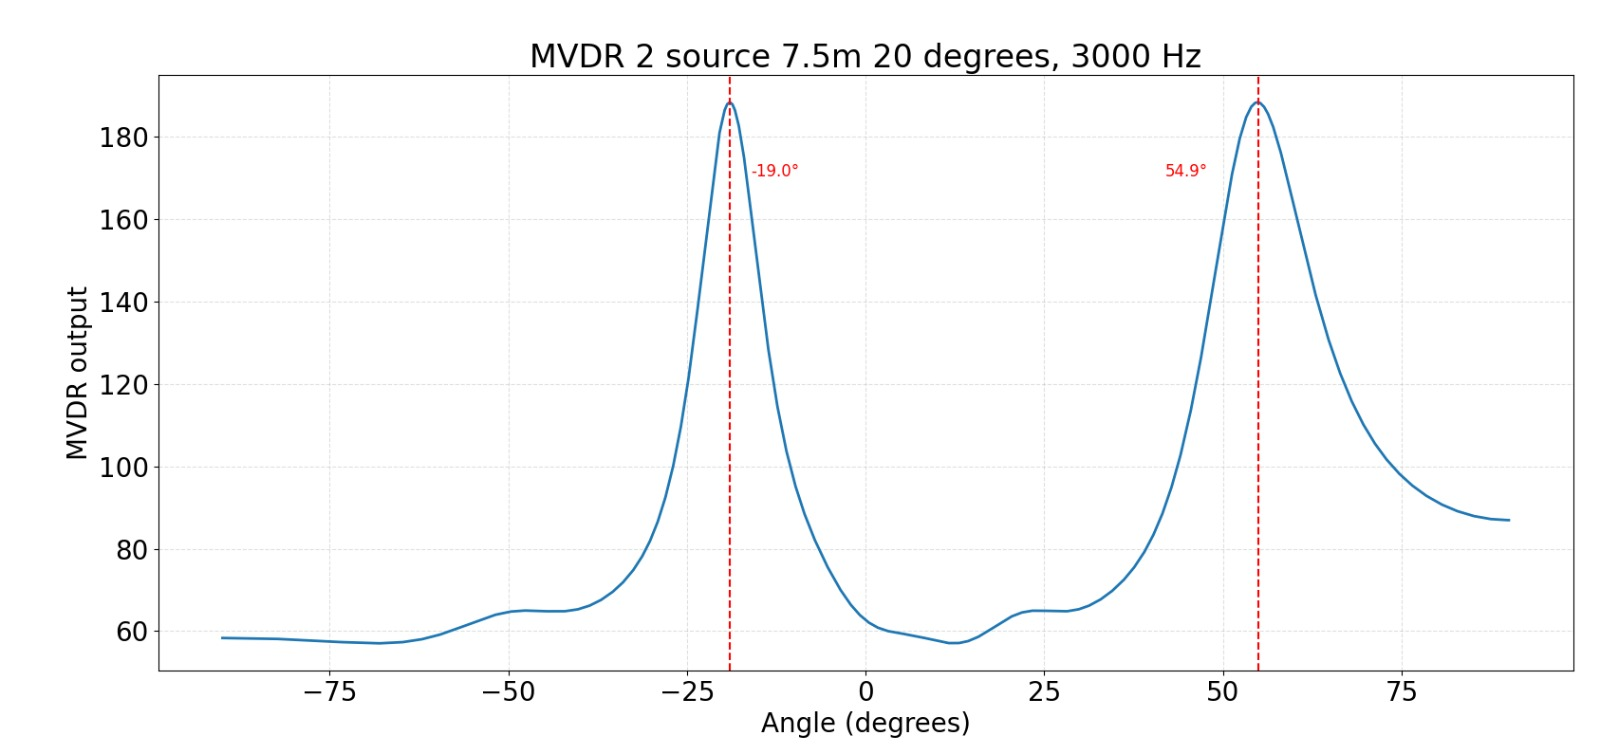
\includegraphics[width=0.8\textwidth]{docs/assignments/Midterm report/figures/MVDR/2 source/20 degrees.jpg}
    \caption{}  
    \label{fig:MVDR4}
\end{figure}

\begin{figure} [H]
    \centering
    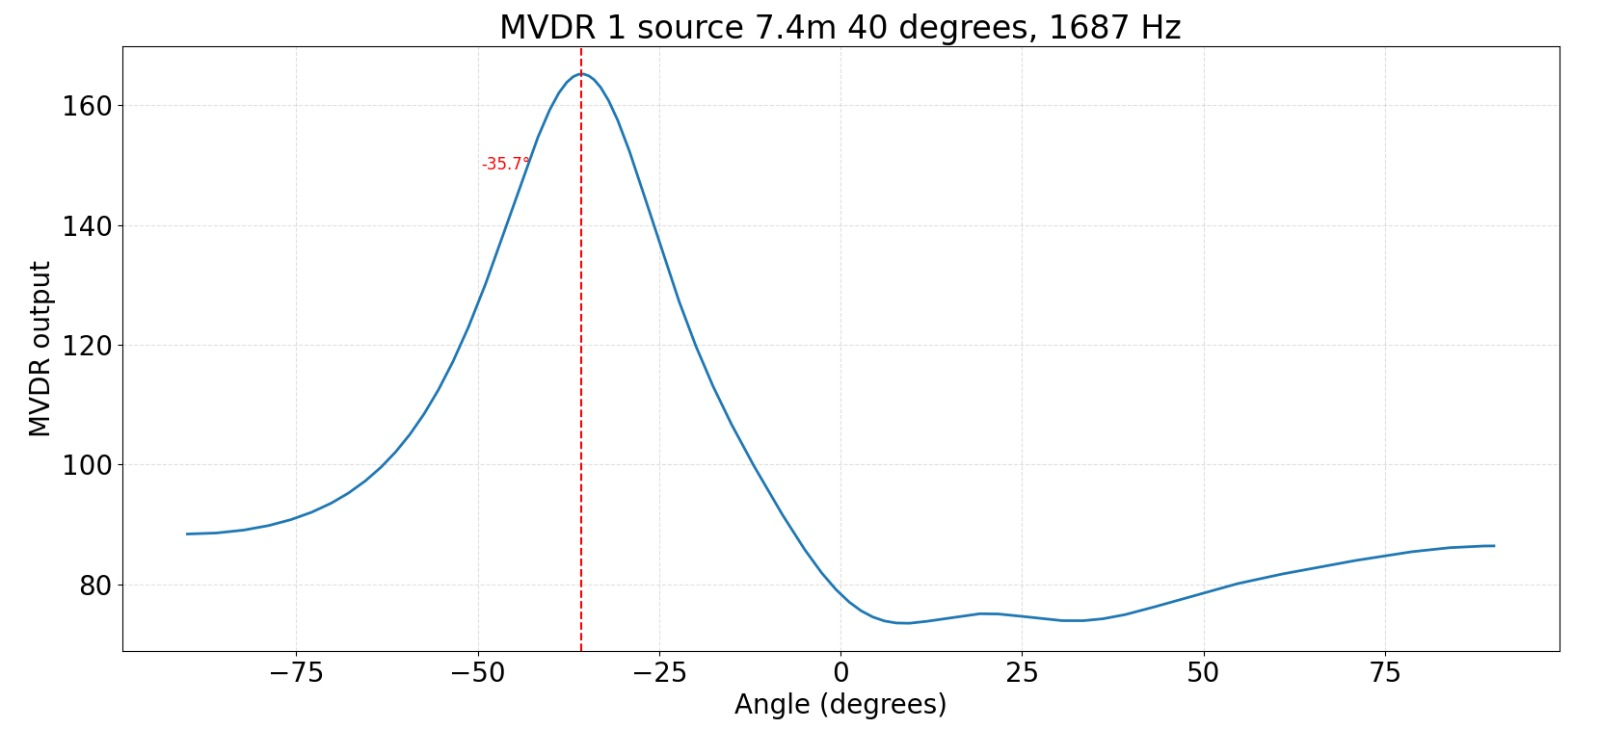
\includegraphics[width=0.8\textwidth]{docs/assignments/Midterm report/figures/MVDR/1 source/40 degrees.jpg}
    \caption{}  
    \label{fig:MVDR5}
\end{figure}

\begin{figure} [H]
    \centering
    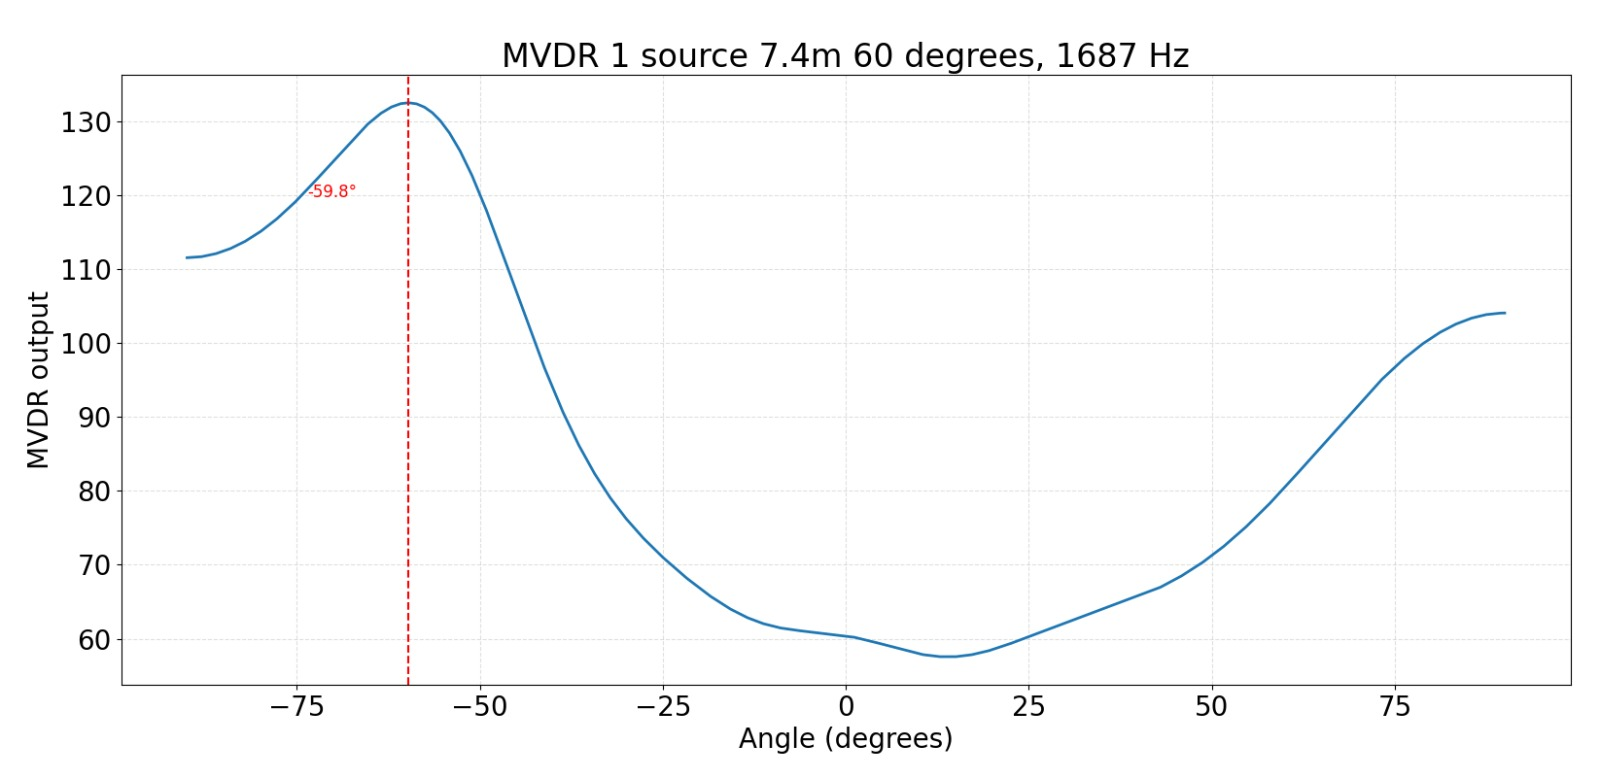
\includegraphics[width=0.8\textwidth]{docs/assignments/Midterm report/figures/MVDR/1 source/60 degrees.jpg}
    \caption{}  
    \label{fig:MVDR6}
\end{figure}

\subsection{Module 4 recordings}

\begin{figure} [H]
    \centering
    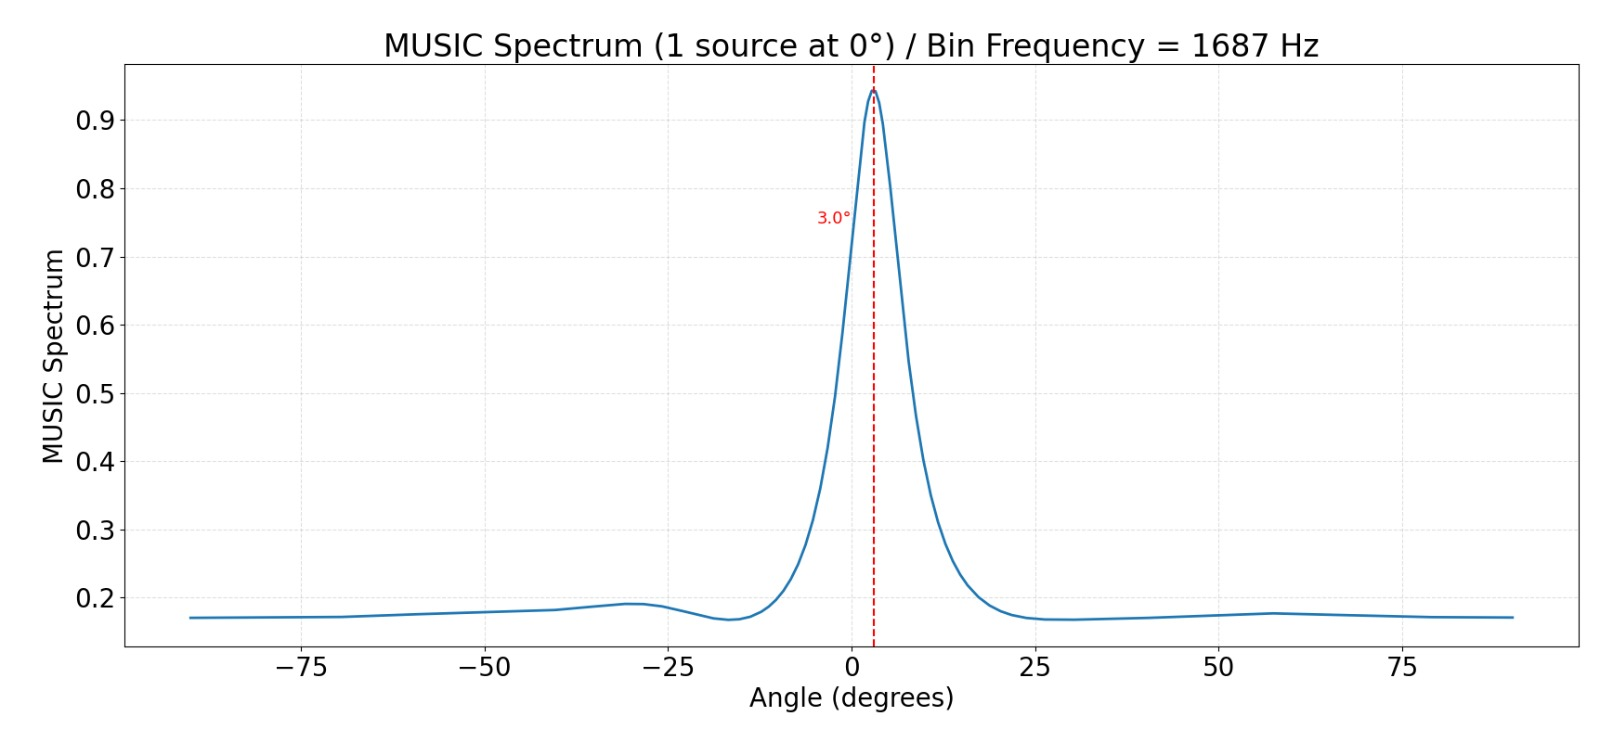
\includegraphics[width=0.8\textwidth]{docs/assignments/Midterm report/figures/MUSIC/1 source/0 degrees.jpg}
    \caption{}  
    \label{fig:MUSIC1}
\end{figure}

\begin{figure} [H]
    \centering
    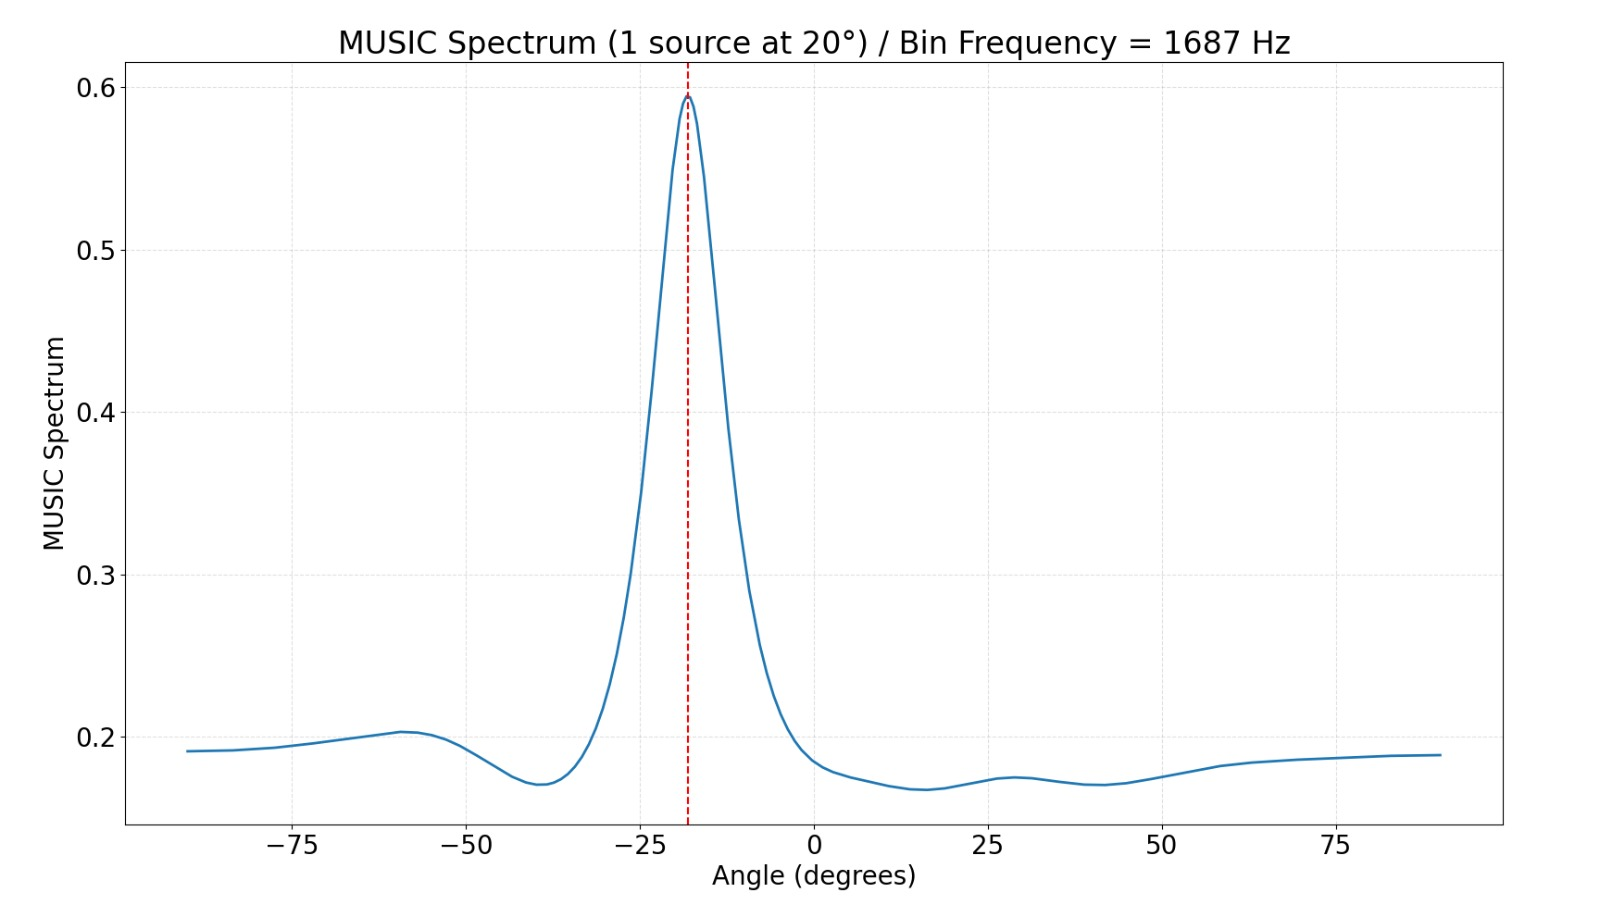
\includegraphics[width=0.8\textwidth]{docs/assignments/Midterm report/figures/MUSIC/1 source/20 degrees.jpg}
    \caption{}  
    \label{fig:MUSIC2}
\end{figure}

\begin{figure} [H]
    \centering
    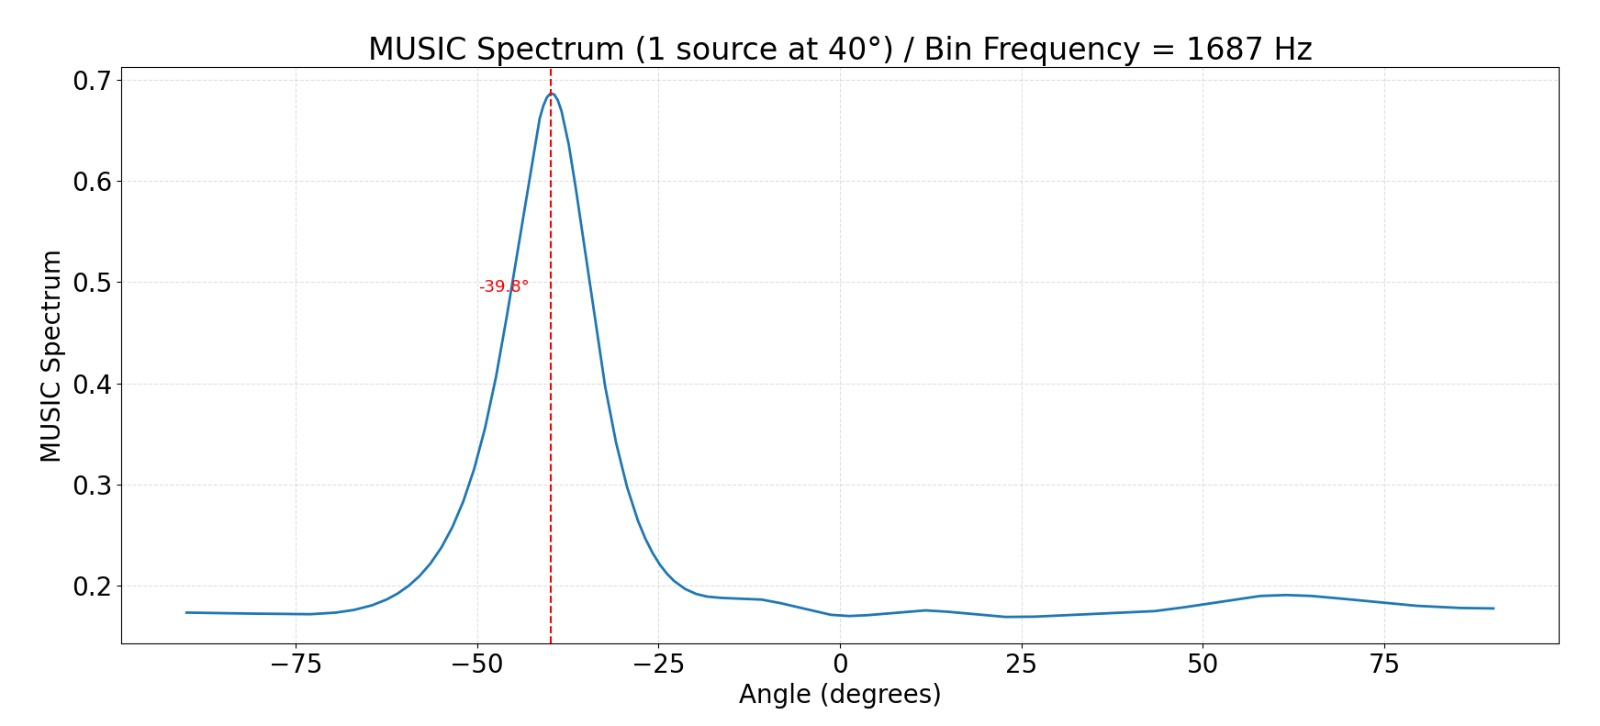
\includegraphics[width=0.8\textwidth]{docs/assignments/Midterm report/figures/MUSIC/1 source/40 degrees.jpg}
    \caption{}  
    \label{fig:MUSIC3}
\end{figure}

\begin{figure} [H]
    \centering
    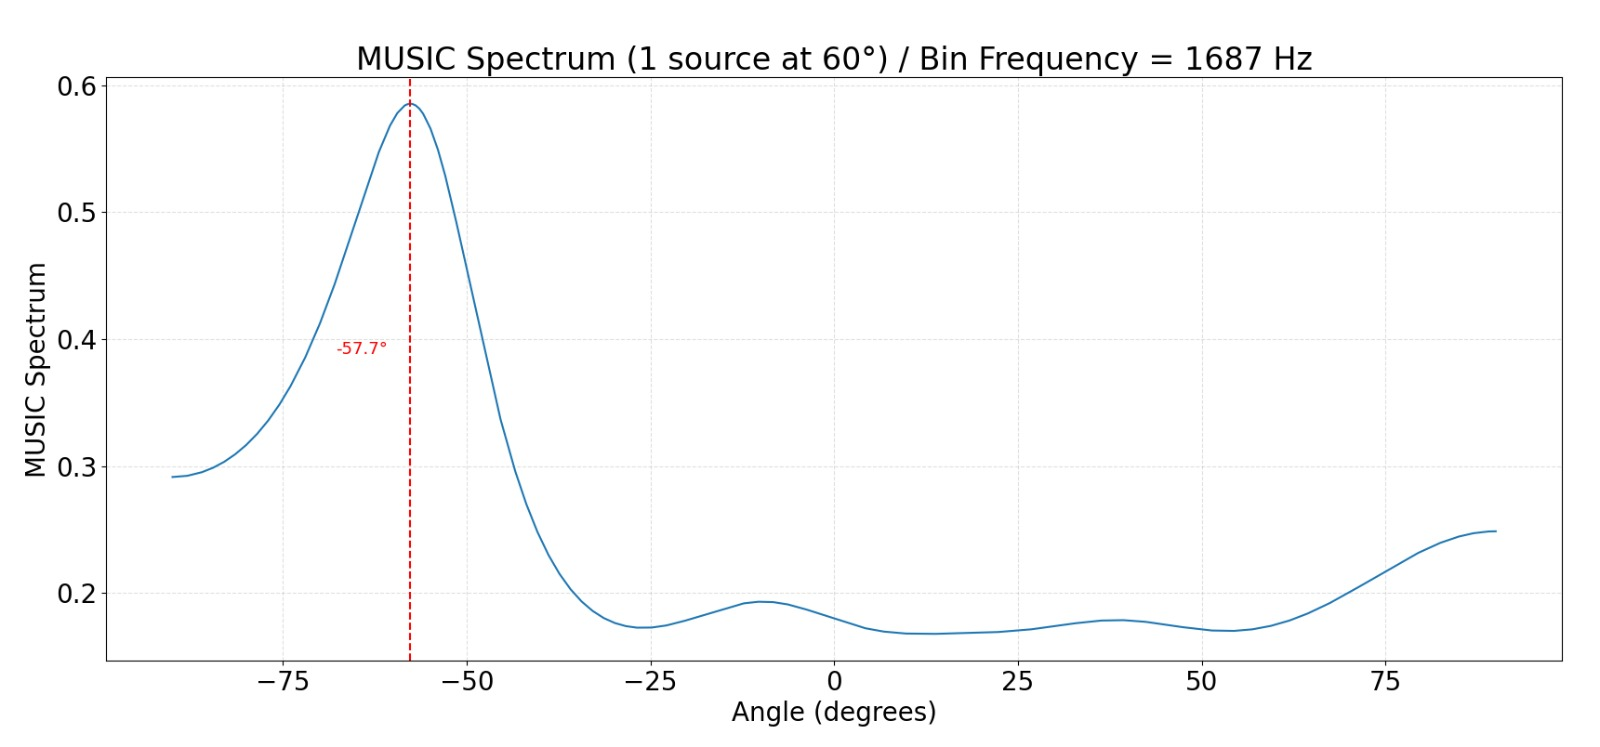
\includegraphics[width=0.8\textwidth]{docs/assignments/Midterm report/figures/MUSIC/1 source/60 degrees.jpg}
    \caption{}  
    \label{fig:MUSIC4}
\end{figure}

\begin{figure} [H]
    \centering
    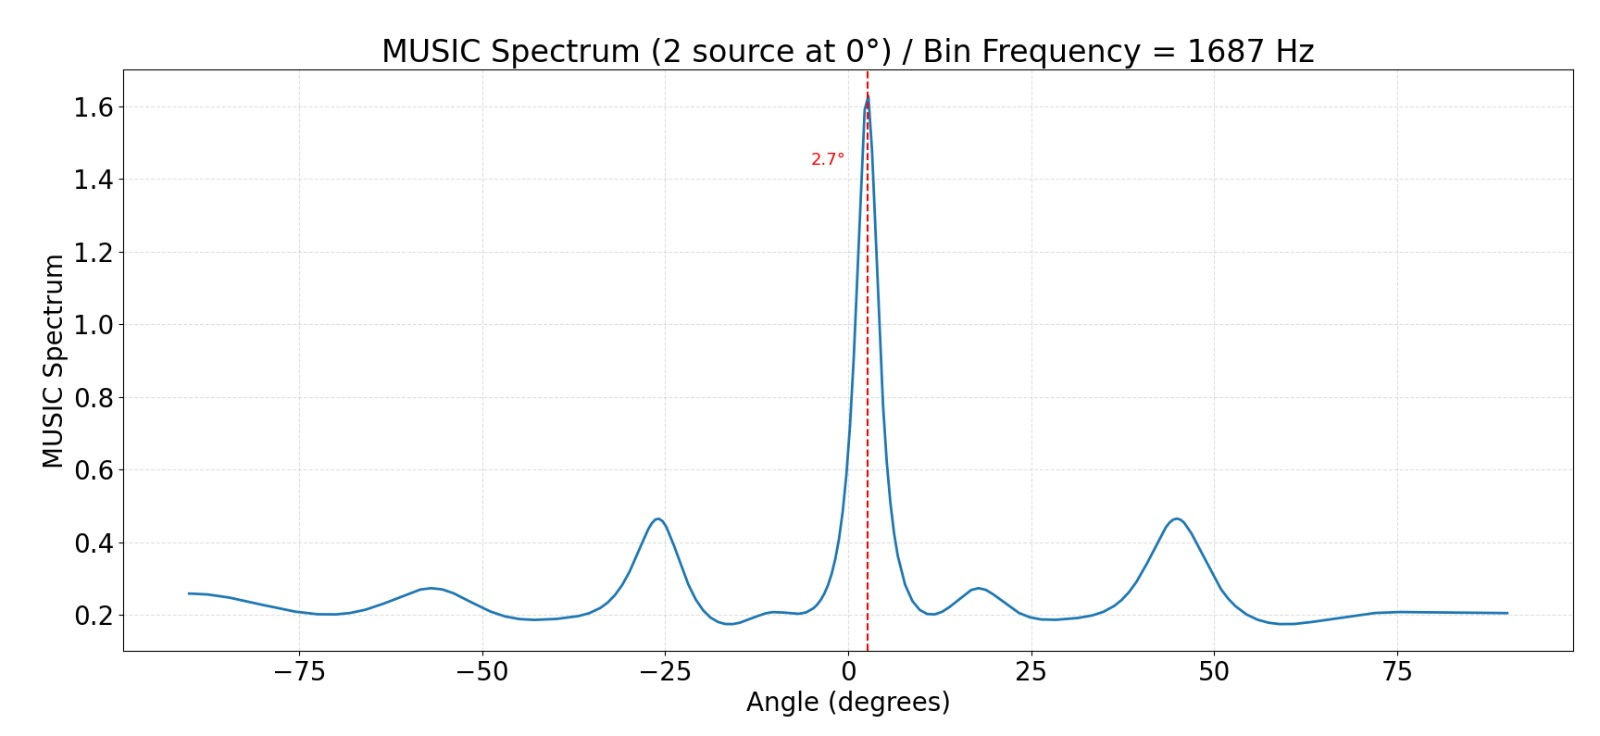
\includegraphics[width=0.8\textwidth]{docs/assignments/Midterm report/figures/MUSIC/2 source/0 degrees.jpg}
    \caption{}  
    \label{fig:MUSIC5}
\end{figure}

\begin{figure} [H]
    \centering
    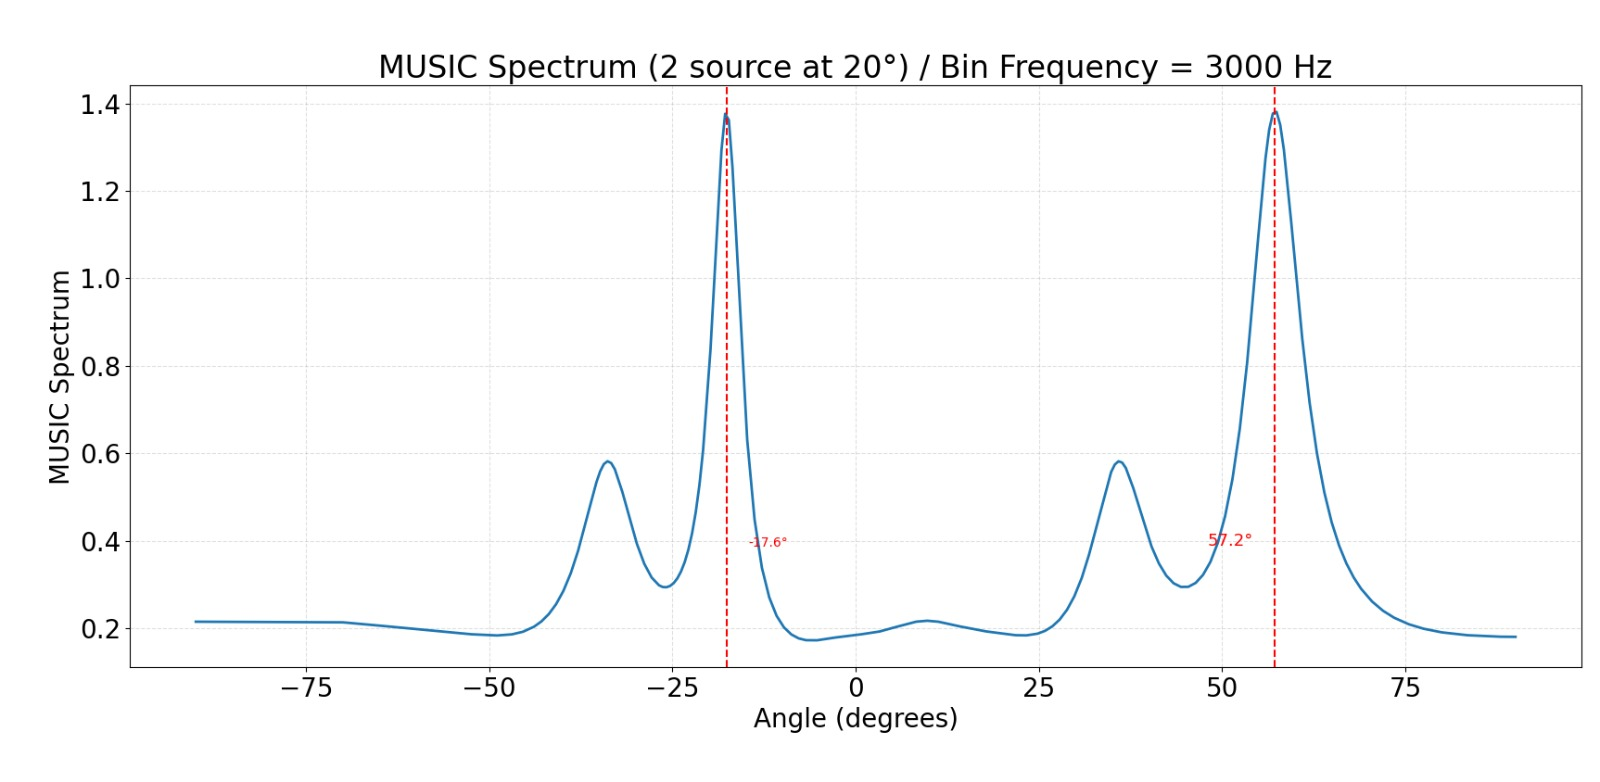
\includegraphics[width=0.8\textwidth]{docs/assignments/Midterm report/figures/MUSIC/2 source/20 degrees.jpg}
    \caption{}  
    \label{fig:MUSIC6}
\end{figure}

\begin{figure} [H]
    \centering
    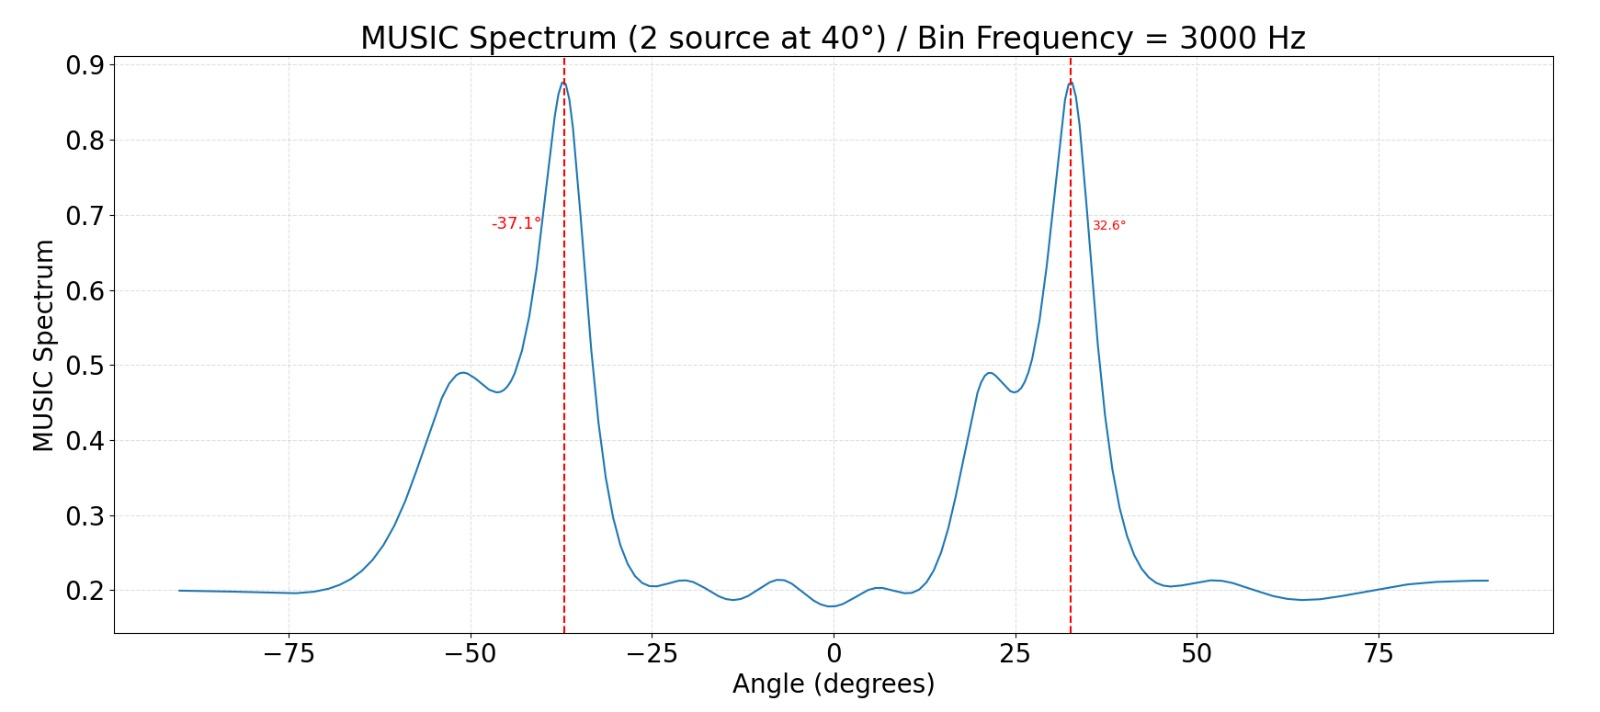
\includegraphics[width=0.8\textwidth]{docs/assignments/Midterm report/figures/MUSIC/2 source/40 degrees.jpg}
    \caption{}  
    \label{fig:MUSIC7}
\end{figure}

\begin{figure} [H]
    \centering
    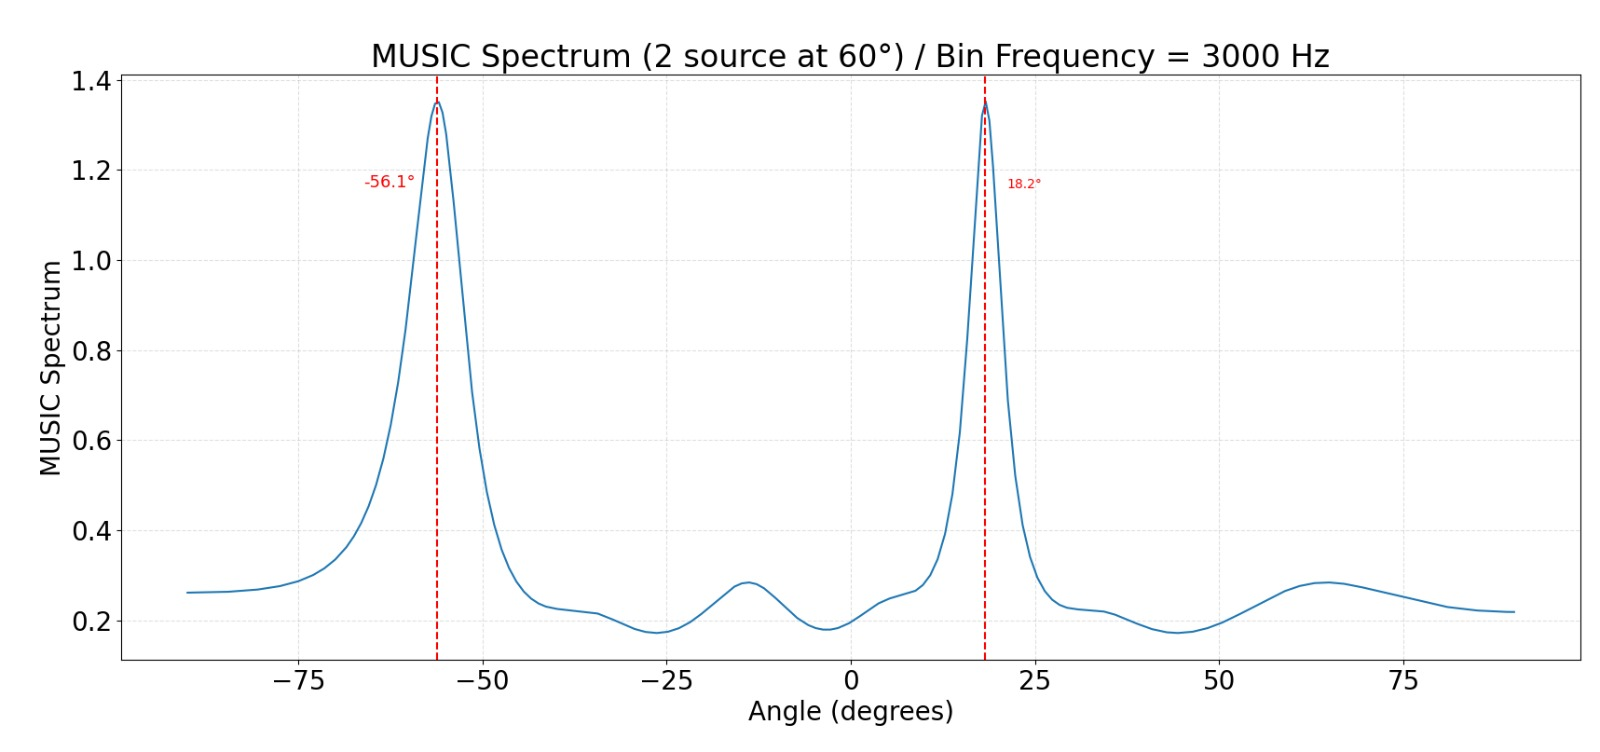
\includegraphics[width=0.8\textwidth]{docs/assignments/Midterm report/figures/MUSIC/2 source/60 degrees.jpg}
    \caption{}  
    \label{fig:MUSIC8}
\end{figure}



